% !TEX root = Tesi.tex
\chead{}
\chapter{Data acquisition}

The evolution of the Internet and the amount of data available from web usage mining and IoT devices have led to an enormous proliferation of the accessible information as per described in the previous sections.  In this chapter, we focus on describing the possible channels of adquisition of customer behavioral data in both the virtual and the physical world. This valuable information represents the milestone of the journey towards the enhancement of the eCommerce experience for its users, and aims at addressing some of the weaknesses of the standard approaches for web personalization.

Before we can efficiently represent content visualized on user interfaces, navigation paths and user-triggered events on a web application, we need to take a little detour briefly introudicing a standard modeling language able to shape such interactions. This language will be analysed in detail in the following sections.

\section{The IFML language}
\label{the-ifml-language}

The Interaction Flow Modeling Language (IFML)\cite{IFML-1, IFML-2} is designed for describing and controlling the behavior of front-end software applications. IFML brings several advantages to the development process, such as promoting the separation of concerns between roles and increasing the overall understanding of the product for non-technical stakeholders. That can be achieved because IFML supports formal specification for interface composition, user interaction and event management independently of the implementation platform. This language was adopted as a standard by the Object Management Group (OMG) in March 2013.

IFML supports the following concepts: 

\begin{itemize}
  \item \textbf{The view structure} describes \textit{ViewContainers}, their nesting relationships, their visibility, and their reachability.
    
  \item \textbf{The view content} manages \textit{ViewComponents}, i.e., content and data entry elements contained within ViewContainers.
  
  \item \textbf{The events} defines the \textit{Events} that may affect the state of the user interface. \textit{Events} can be produced by the user interaction, by the application, or by an external system.

  \item \textbf{The actions} triggered by user events. The effect of an \textit{Event} is represented by an \textit{InteractionFlow} connection, which connects the event to the \textit{ViewContainer} or \textit{ViewComponent} affected by the \textit{Event}. The \textit{InteractionFlow} expresses a change of state of the user interface: the occurrence of the event triggers a change in the state that produces a transition in the user interface.
  
  \item \textbf{The navigation flow} indicates the effect of an Event on the user interface.

  \item \textbf{The data flow} indicates the data passed between \textit{ViewComponents} and \textit{Actions}.
  
  \item \textbf{The parameter binding} illustrates the input-output dependencies between \textit{ViewComponents} and between \textit{ViewComponents} and \textit{Actions}. 


\end{itemize} 

\vspace{0.5cm}
\begin{figure}[H]
  \centering
    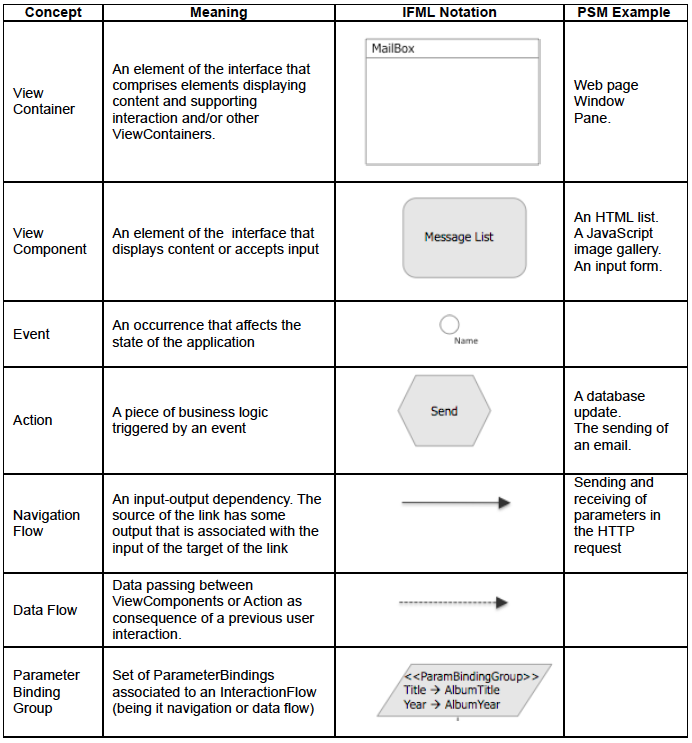
\includegraphics[width=10cm]{images/ifml.jpg}
  \caption{Main IFML concepts and notations.}
  \label{fig:ifml}
\end{figure}
\vspace{0.5cm}

\newpage

\section{Web navigation profiling}
\label{navigational-modeling-for-the-web}
The front-end of eCommerce websites is usually built using shared and reusable components (forms, list views, detail views, etc.), which have a specific and expected behavior.
For example, product lists and grids show users record details and create possibilities for interaction. Similarly, "add to cart" buttons are placed on strategic points within product pages to trigger a specific user action.
These interactions and any other user action withing the website can be represented using the IFML notation.

To demonstrate the versatility and adaptability of this modeling language, we introduce a real-life example which will serve as reference from this chapter forward: an online boutique website called \textit{"Madison Island"} and specialized in fashion items running on an eCommerce platform.

Madison Island presents all the features of a typical digital store including catalog navigation, product searching, customer account, shopping cart, and order processing. 

\vspace{0.5cm}
\begin{figure}[htbp]
  \centering
    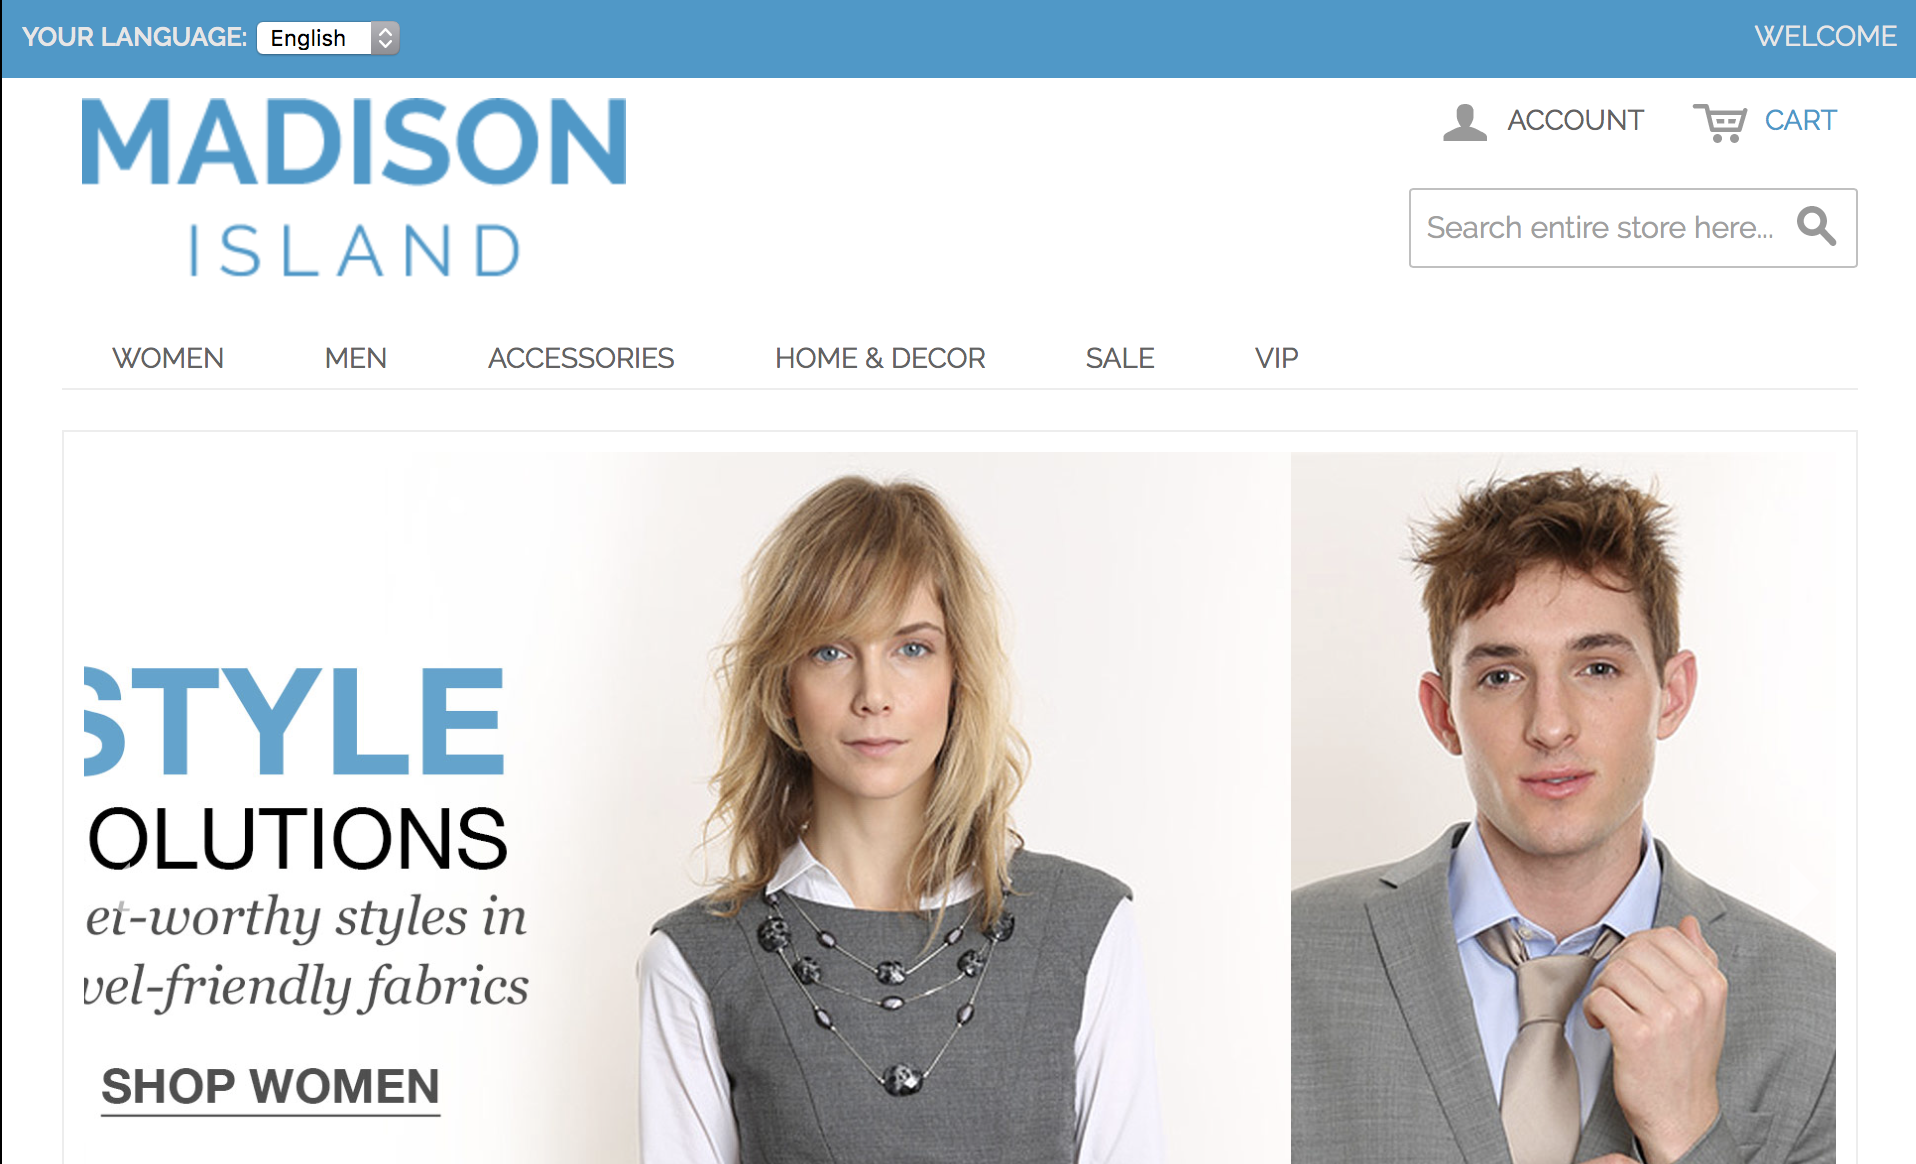
\includegraphics[width=12cm]{images/home.png}
  \caption{Madison Island digital store homepage}
  \label{fig:home}
\end{figure}
\vspace{0.5cm}


Figure \ref{fig:home} shows the home page of the website. In this section, the user can select one of the product categories, access his customer area, switch the language of the website, search for an item or go directly to the shopping cart. 

In the following subsections, we analyse some scenarios related to users navigational behaviors, exposing both their representation in IFML notation as well as the log entries in the application server associated with those representations.

\newpage
\subsection{The product page journey}

Starting from the homepage, the user can interact with the navigation menu by choosing from a set of available categories.  (Figure \ref{fig:navigation})

\vspace{0.5cm}
\begin{figure}[H]
  \centering
    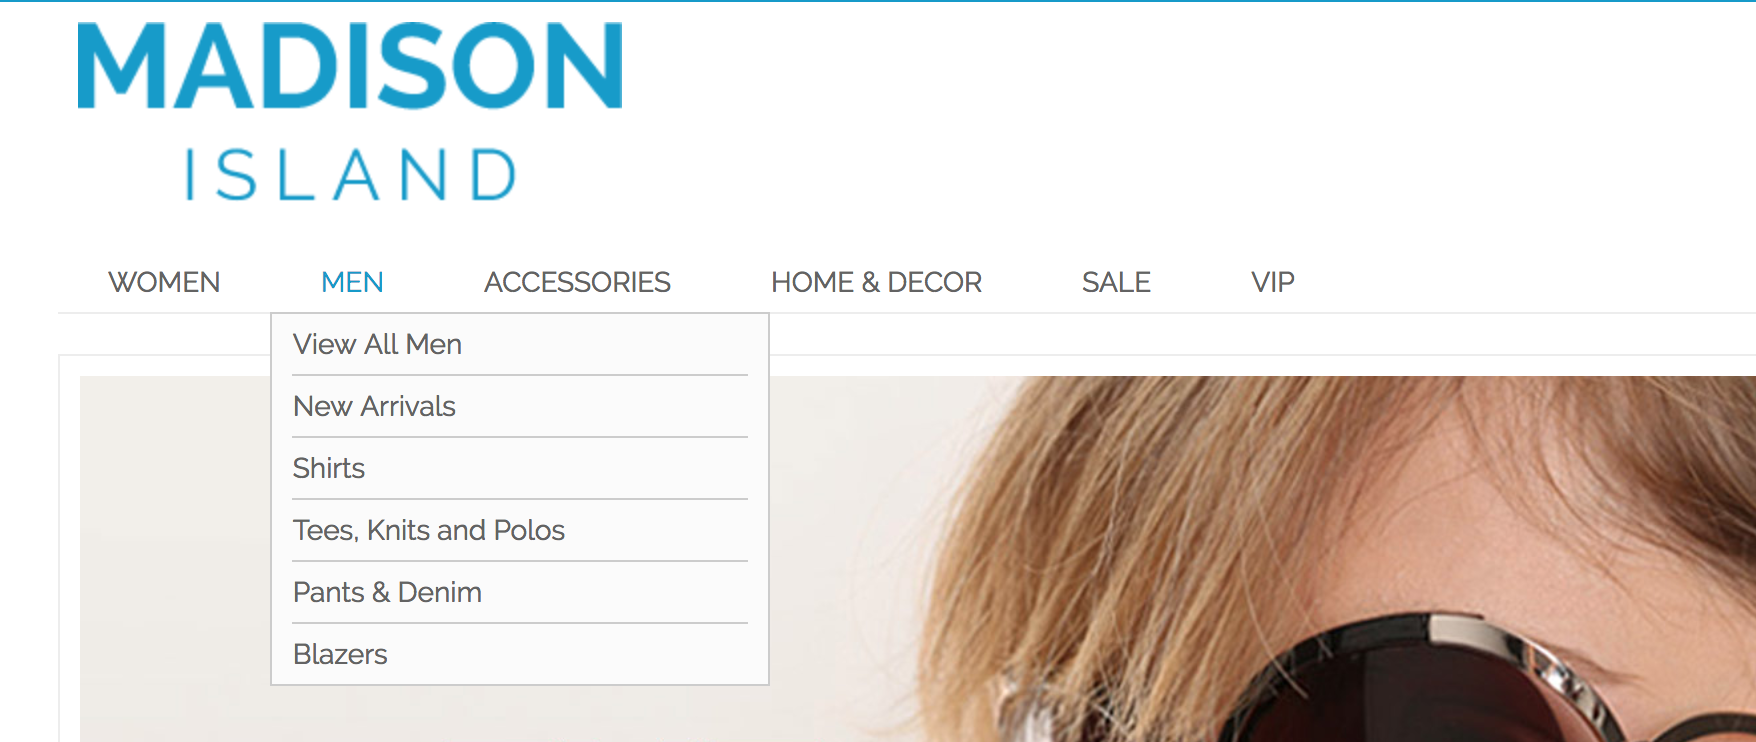
\includegraphics[width=9cm]{images/madison/navigation.png}
  \caption{Navigation menu}
  \label{fig:navigation}
\end{figure}
\vspace{0.5cm}

Depending on the category display mode, a category page can show users either a list of links to children categories or a set of products. The the former case, children categories work as transitional pages that help further filtering products (Figure \ref{fig:category-display-modes}).


\vspace{0.5cm}
\begin{figure}[H]
  \centering
  \subfloat[Category listing]{{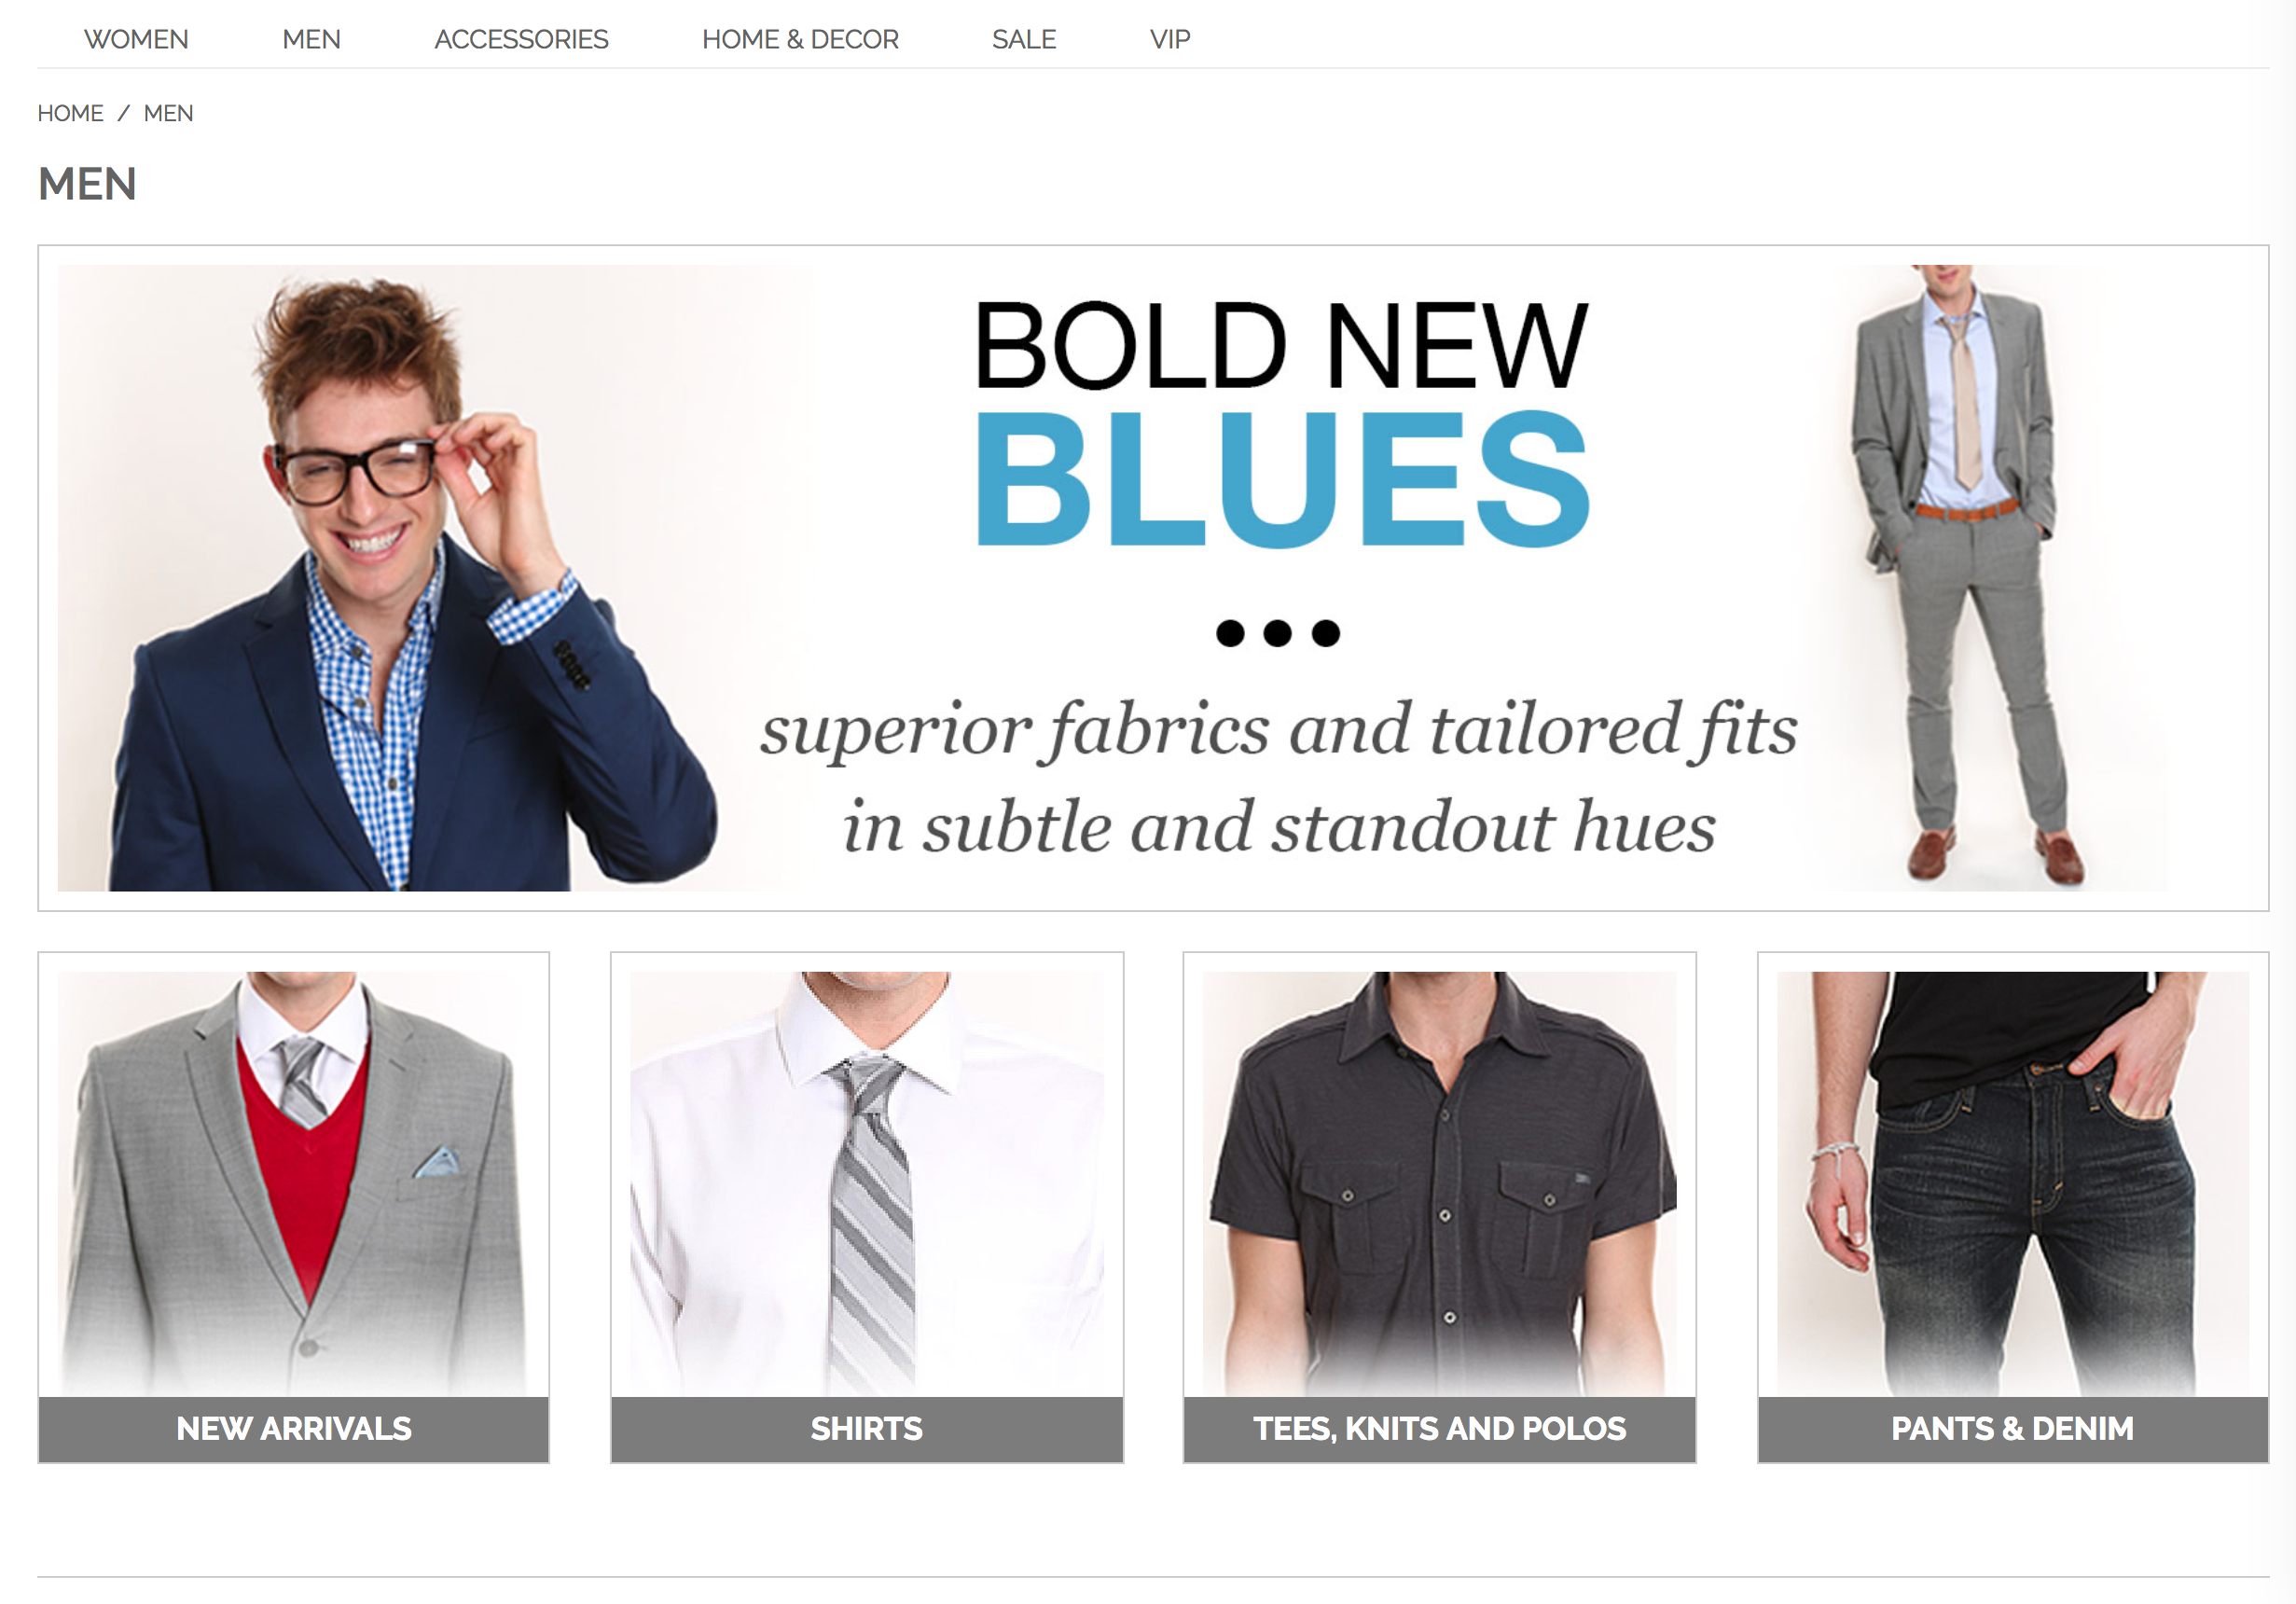
\includegraphics[width=7cm]{images/madison/category-cms.png} }}%
  \qquad
  \subfloat[Product listing]{{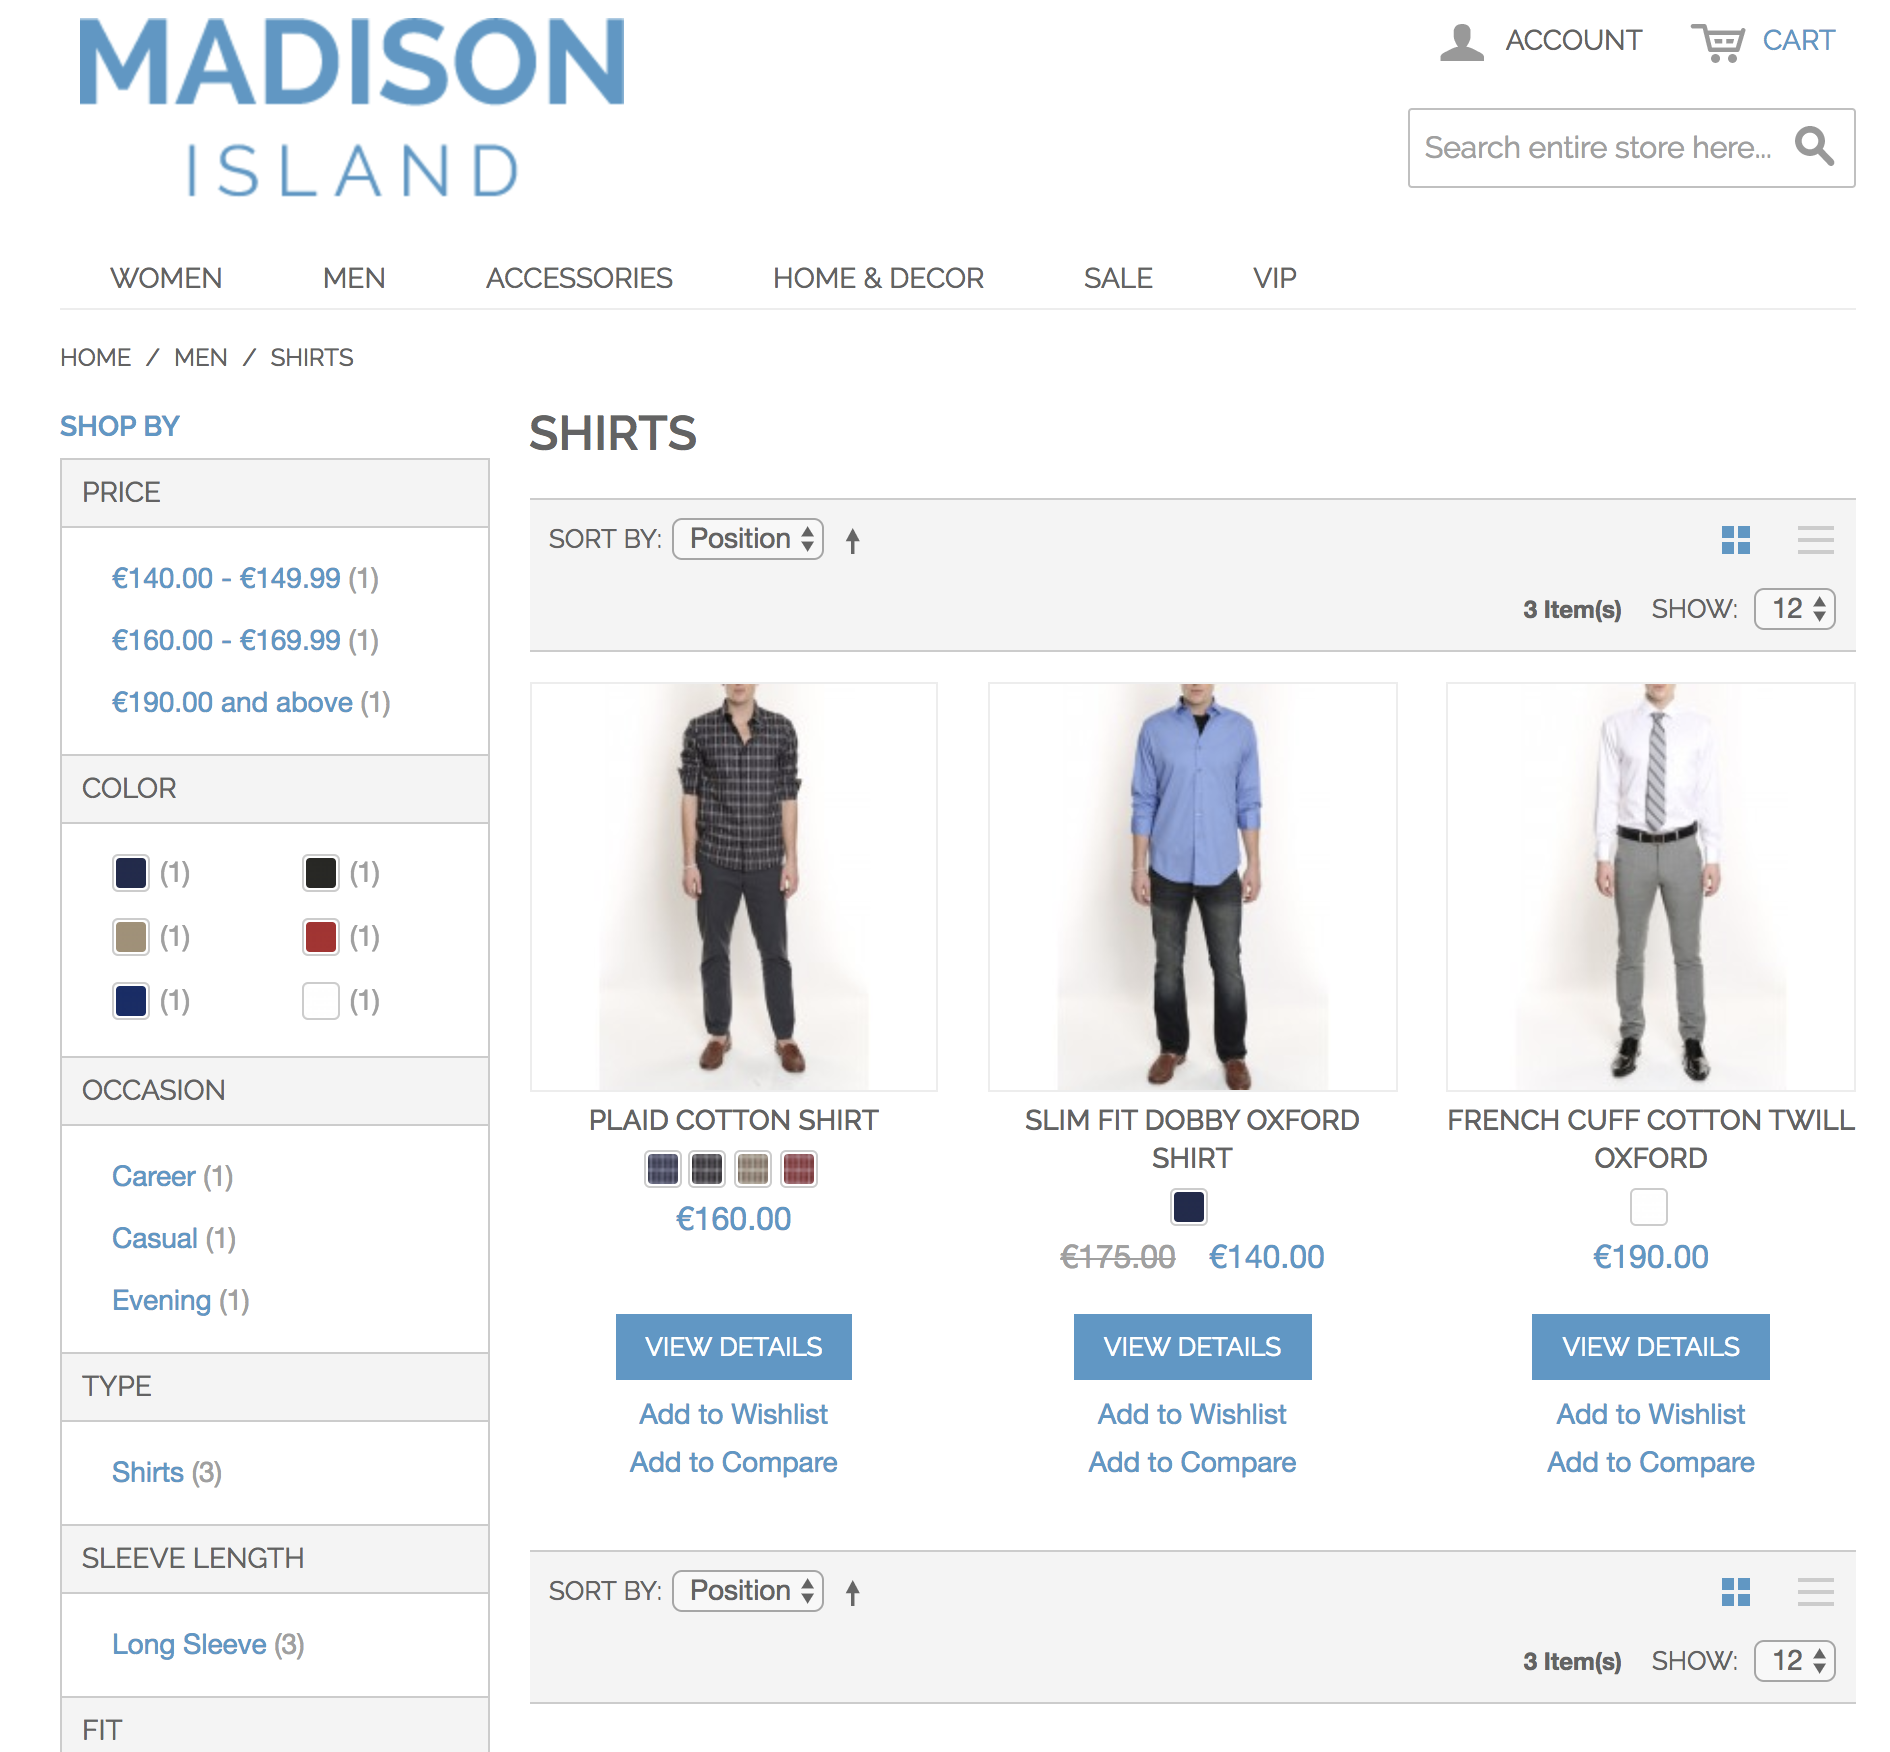
\includegraphics[width=7cm]{images/madison/products-list.png} }}%
  \caption{Different category page view modes}%
  \label{fig:category-display-modes}%
\end{figure}
\vspace{0.5cm}

Finally, from the product listing screen, the user can access any of the product detail pages by clicking on the \textit{"View Details"} button placed below the selected product thumbnail. The following image illustrates the product page seen when the user clicks on \textit{"View Details"} of \textit{"Plaid Cotton Shirt"} (Figure \ref{fig:product-detail}).


\vspace{0.5cm}
\begin{figure}[H]
  \centering
    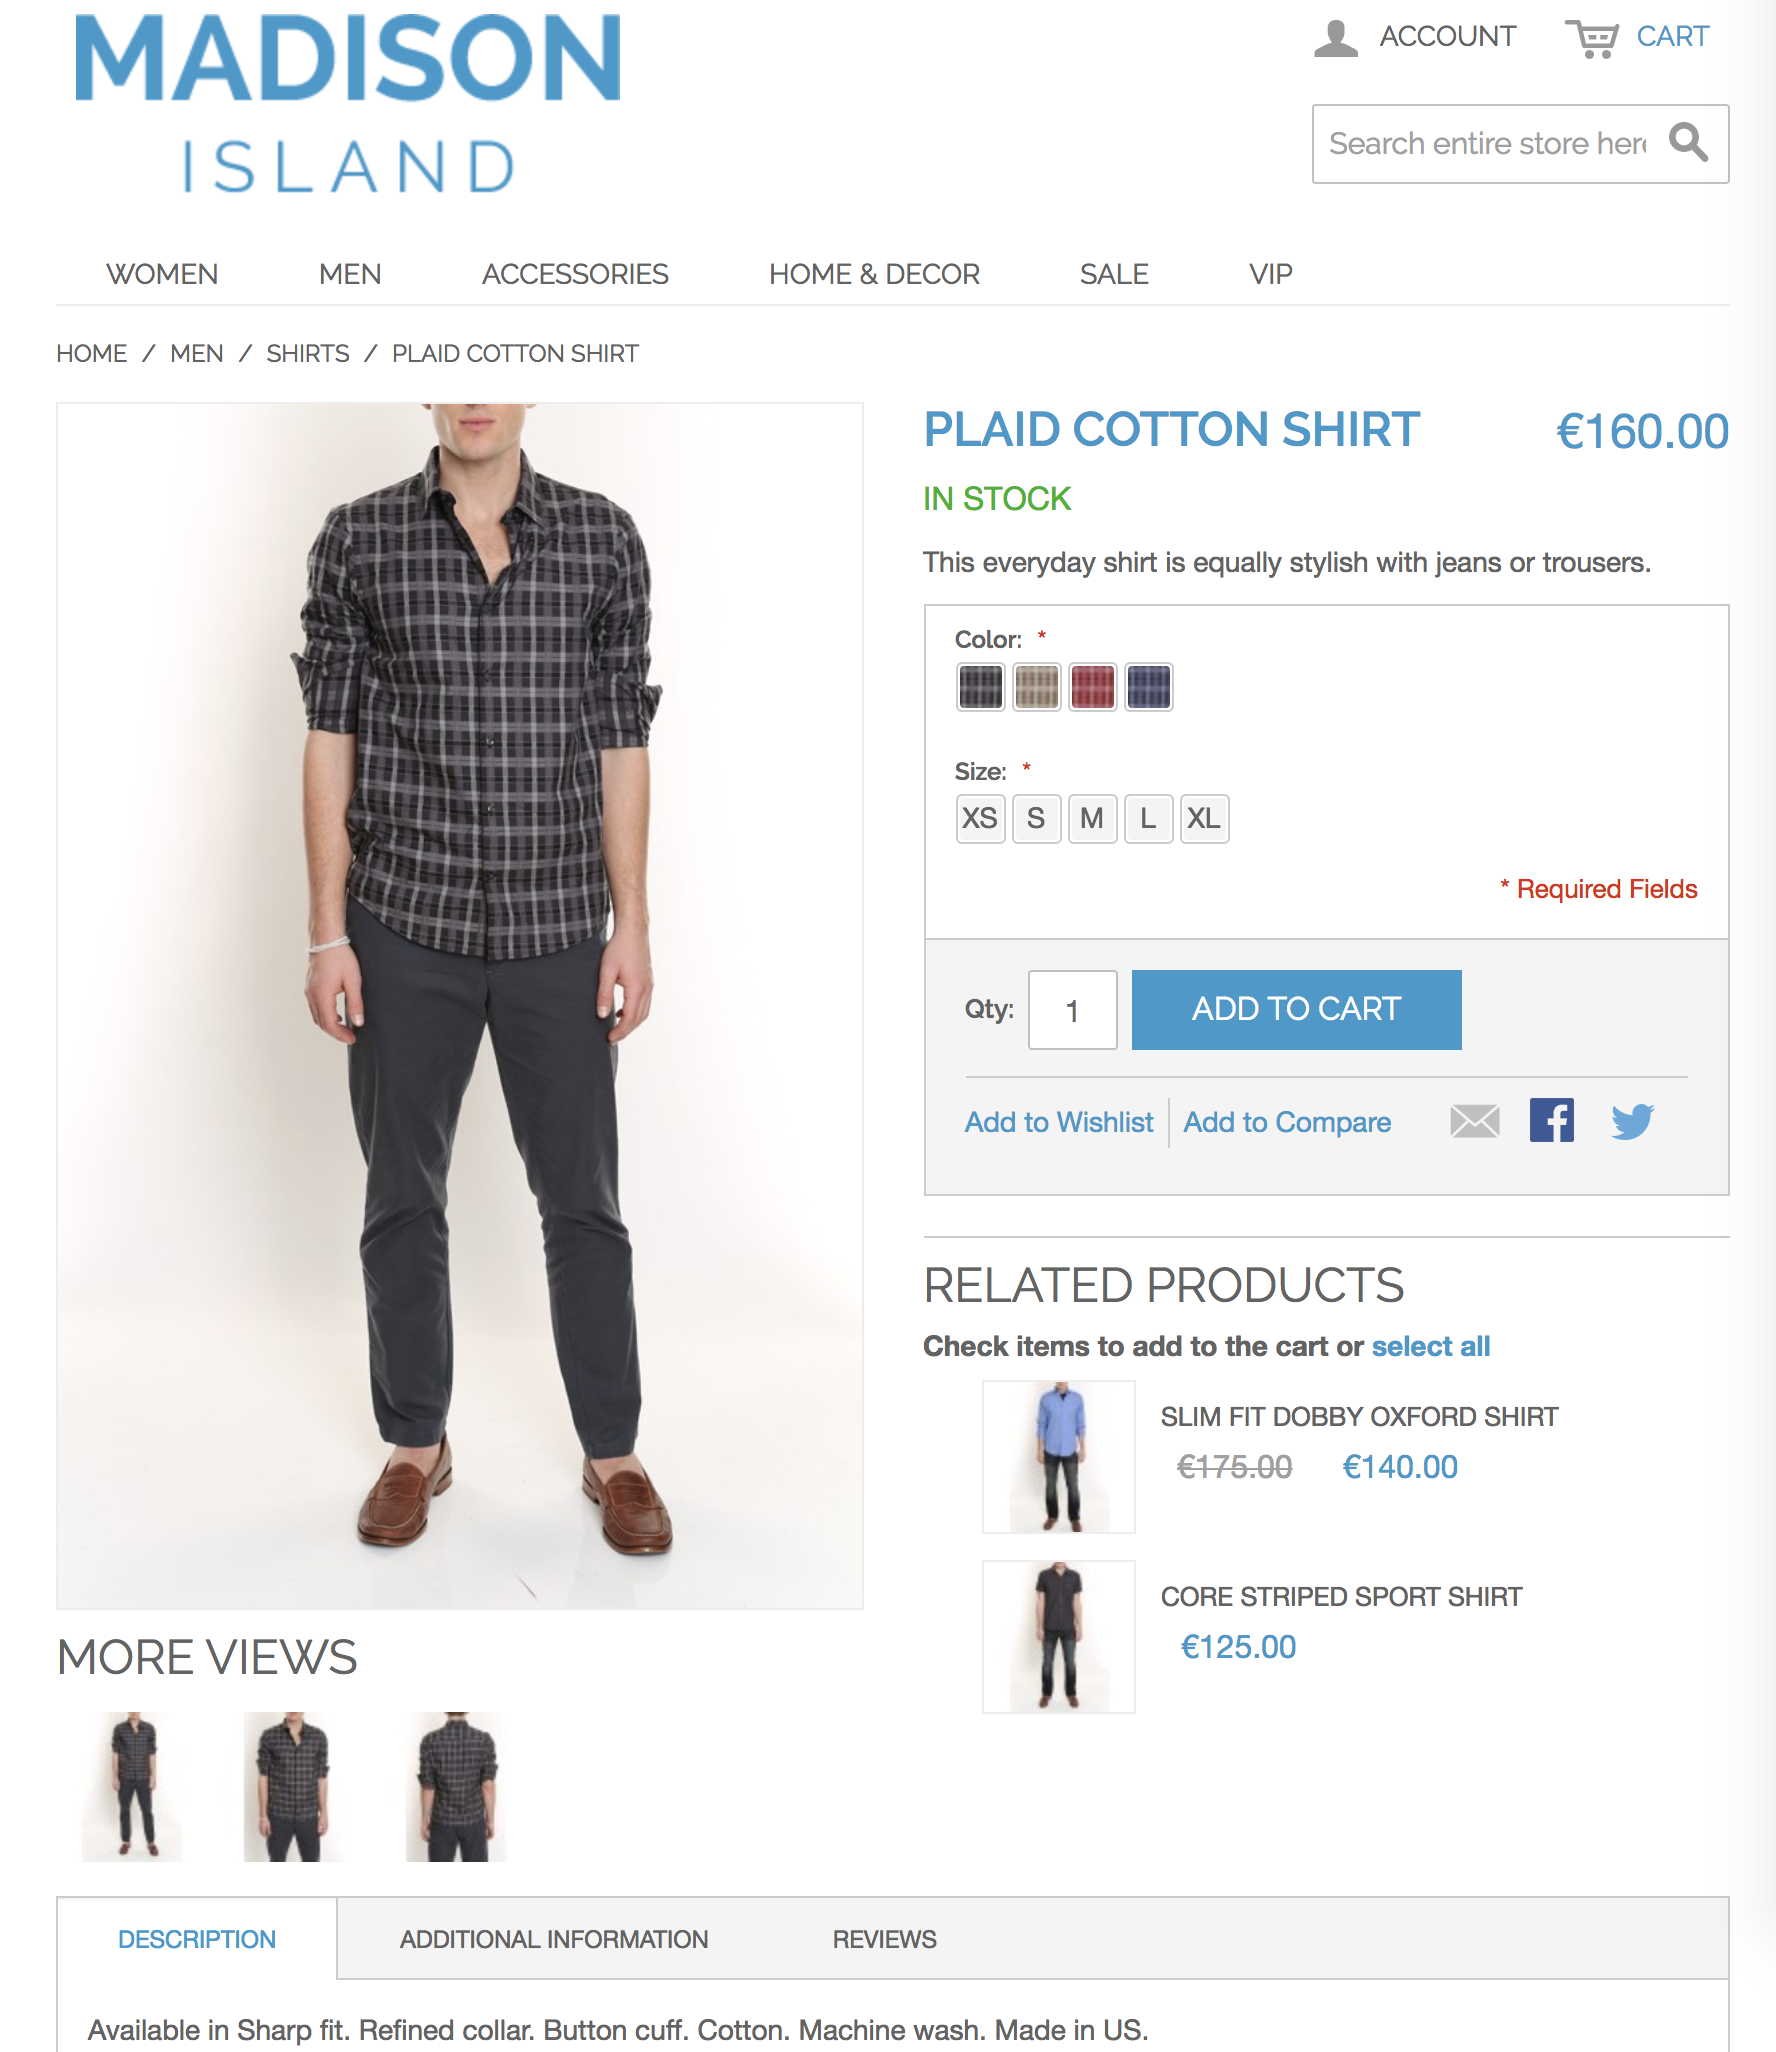
\includegraphics[height=8cm]{images/madison/product-detail.png}
  \caption{Product detail page}
  \label{fig:product-detail}
\end{figure}
\vspace{0.5cm}

The end-to-end interaction from the homepage to the product detail page can be represented by a model using the following IFML notation:

\vspace{0.5cm}
\begin{figure}[H]
  \centering
    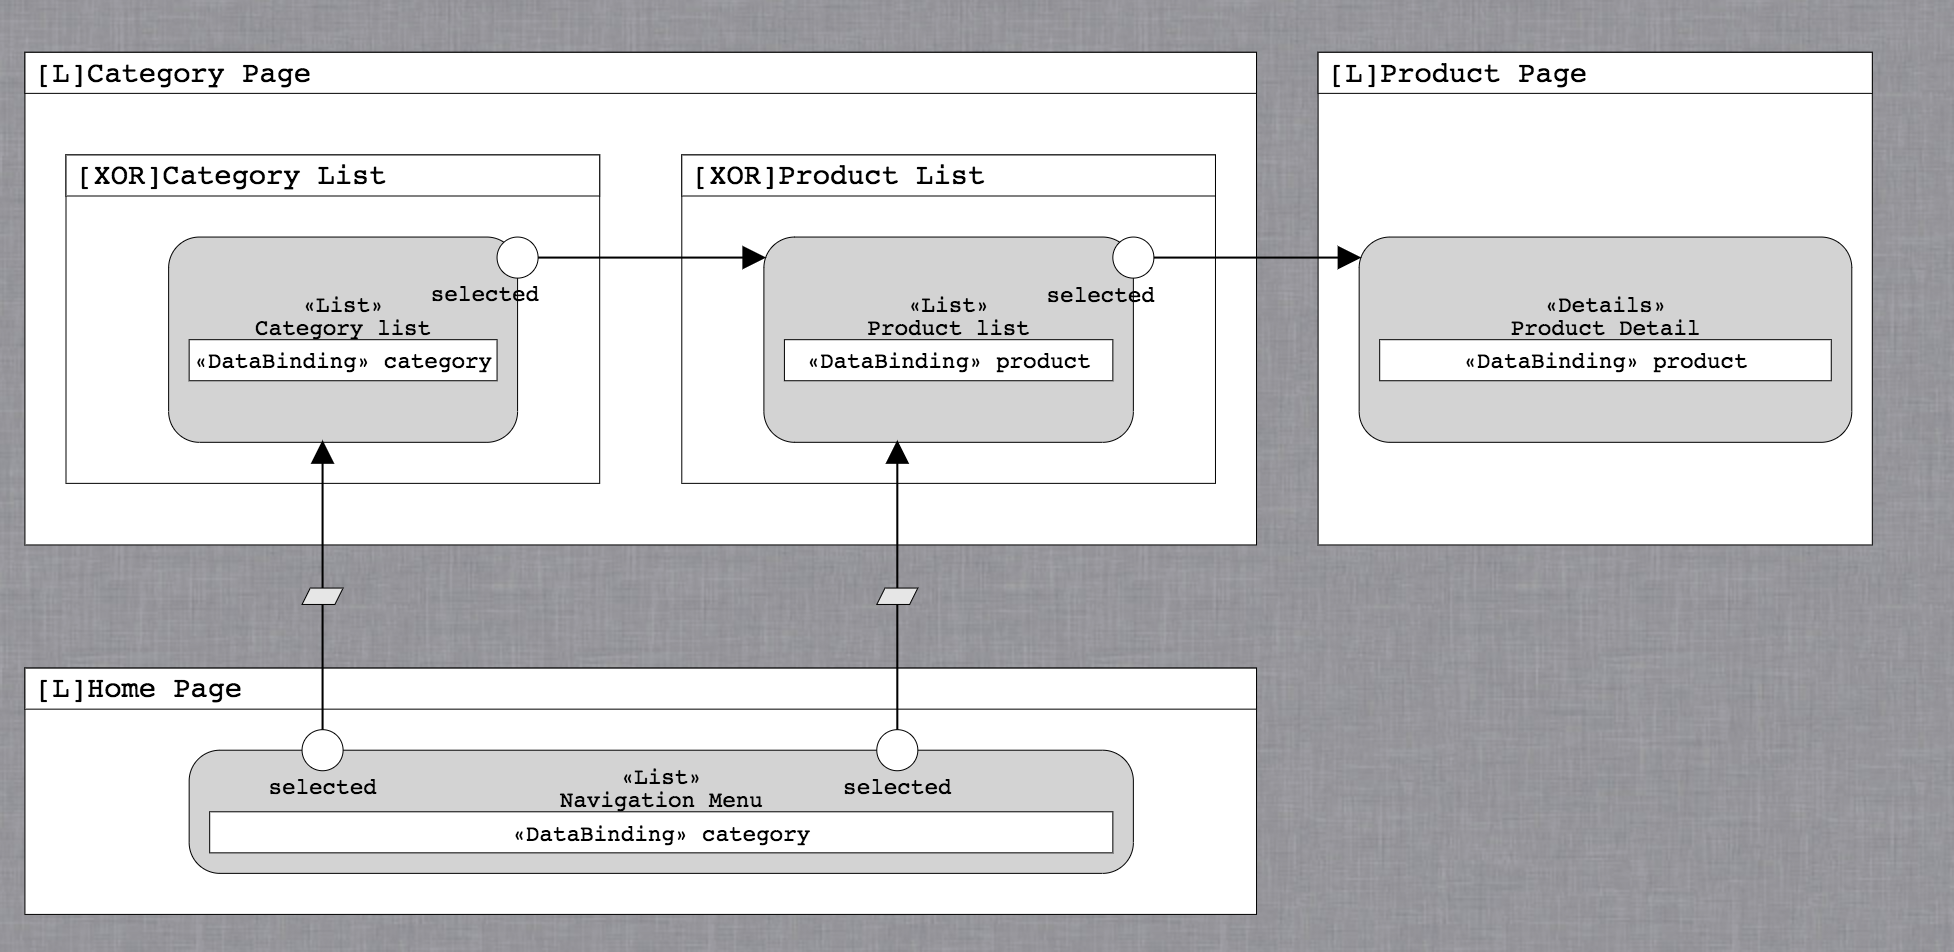
\includegraphics[width=12cm]{images/madison/ifml1.png}
  \caption{IFML representation of the Product Detail interaction}
  \label{fig:ifml1}
\end{figure}
\vspace{0.5cm}

The same sequence of actions can be expressed as a stream of records in the access logs on the application server. Such logs track all the requests processed by the web platform. The following table presents how the above mentioned user journey is logged on the server.

\vspace{0.5cm}
\begin{center}
  \begin{tabular}{|c|p{3cm}|c|p{6cm}|}
  \hline
  \multicolumn{4}{|c|}{Application Server Access Log}\\ \hline
  \textbf{ID}&\textbf{Page}&\textbf{IFML}&\textbf{Log Entry}   \\ \hline
  1&Home Page&Home&\em[29/Nov/2017:06:30:45 +0000] "GET /" 200 0 - 29505 \\ \hline
  2&\textit{"View All Men"} Category Page &Category&\em[29/Nov/2017:06:49:38 +0000] "GET /men.html /" 200 0 - 29505 
  \\ \hline
  3&\textit{"Shirts"} Category Page &Category&\em[29/Nov/2017:07:04:15 +0000] "GET /men/shirts.html" 200 0 - 29505
  \\ \hline
  4&\textit{"Plaid Cotton Shirt"} Product Page &Product&\em[29/Nov/2017:07:08:40 +0000] "GET /men/shirts/plaid-cotton-shirt-476.html" 200 0 - 29505
  \\ \hline
  \end{tabular}
  \end{center}
  \vspace{0.5cm}

  It is important to notice that both entries 2 and 3 record a \textit{"Category Page"} pageview action by logging their related URLs. The entry 4, on its turn, tracks a \textit{"Product Page"} visit by logging a specific URL that concatenates the product URL key and the category path. \textcolor{red}{This concatenation indicates that the product was accessed directly from a category page.}


\subsection{Products association and correlation}

In this section, we analyze the set of actions that can generate pageviews among different product pages on the Madison Island website. 

For doing so, we consider a \textit{"Plaid Cotton Shirt"} widget presented to customers just below the \textit{"Add to Cat"} button on the \textit{"Plaid Cotton Shirt"} discussed on \textcolor{red}{3.2.1}.

\vspace{0.5cm}
\begin{figure}[H]
  \centering
    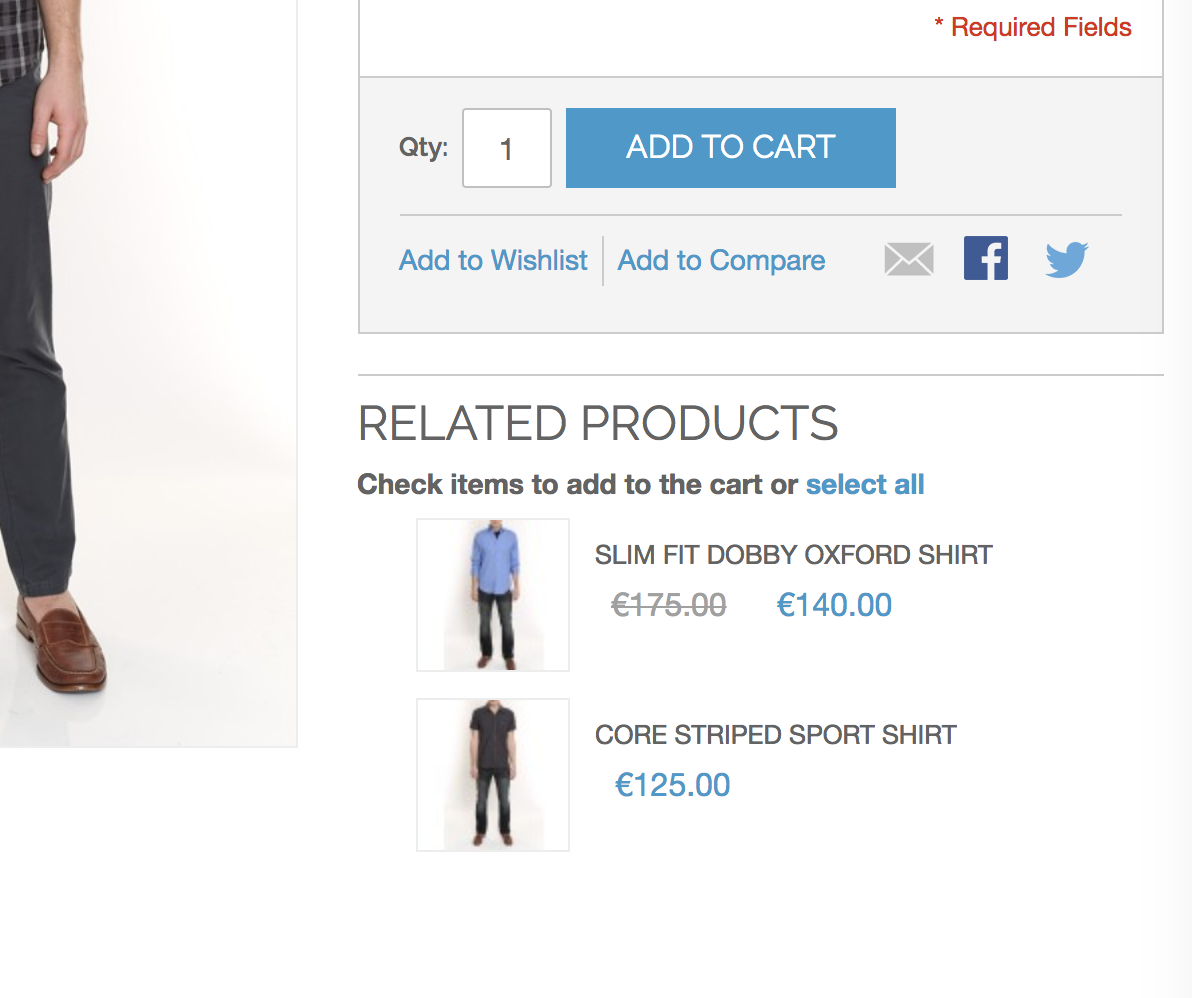
\includegraphics[width=8cm]{images/madison/related-products.png}
  \caption{Related products section}
  \label{fig:related-products}
\end{figure}
\vspace{0.5cm}

By clicking either on the product name or on its thumbnail, the user is directed to the related product page. In this case, we simulate an interest on the listed \textit{"Core Striped Sport Shirt"} (Figure \ref{fig:product-detail2}).

\vspace{0.5cm}
\begin{figure}[H]
  \centering
    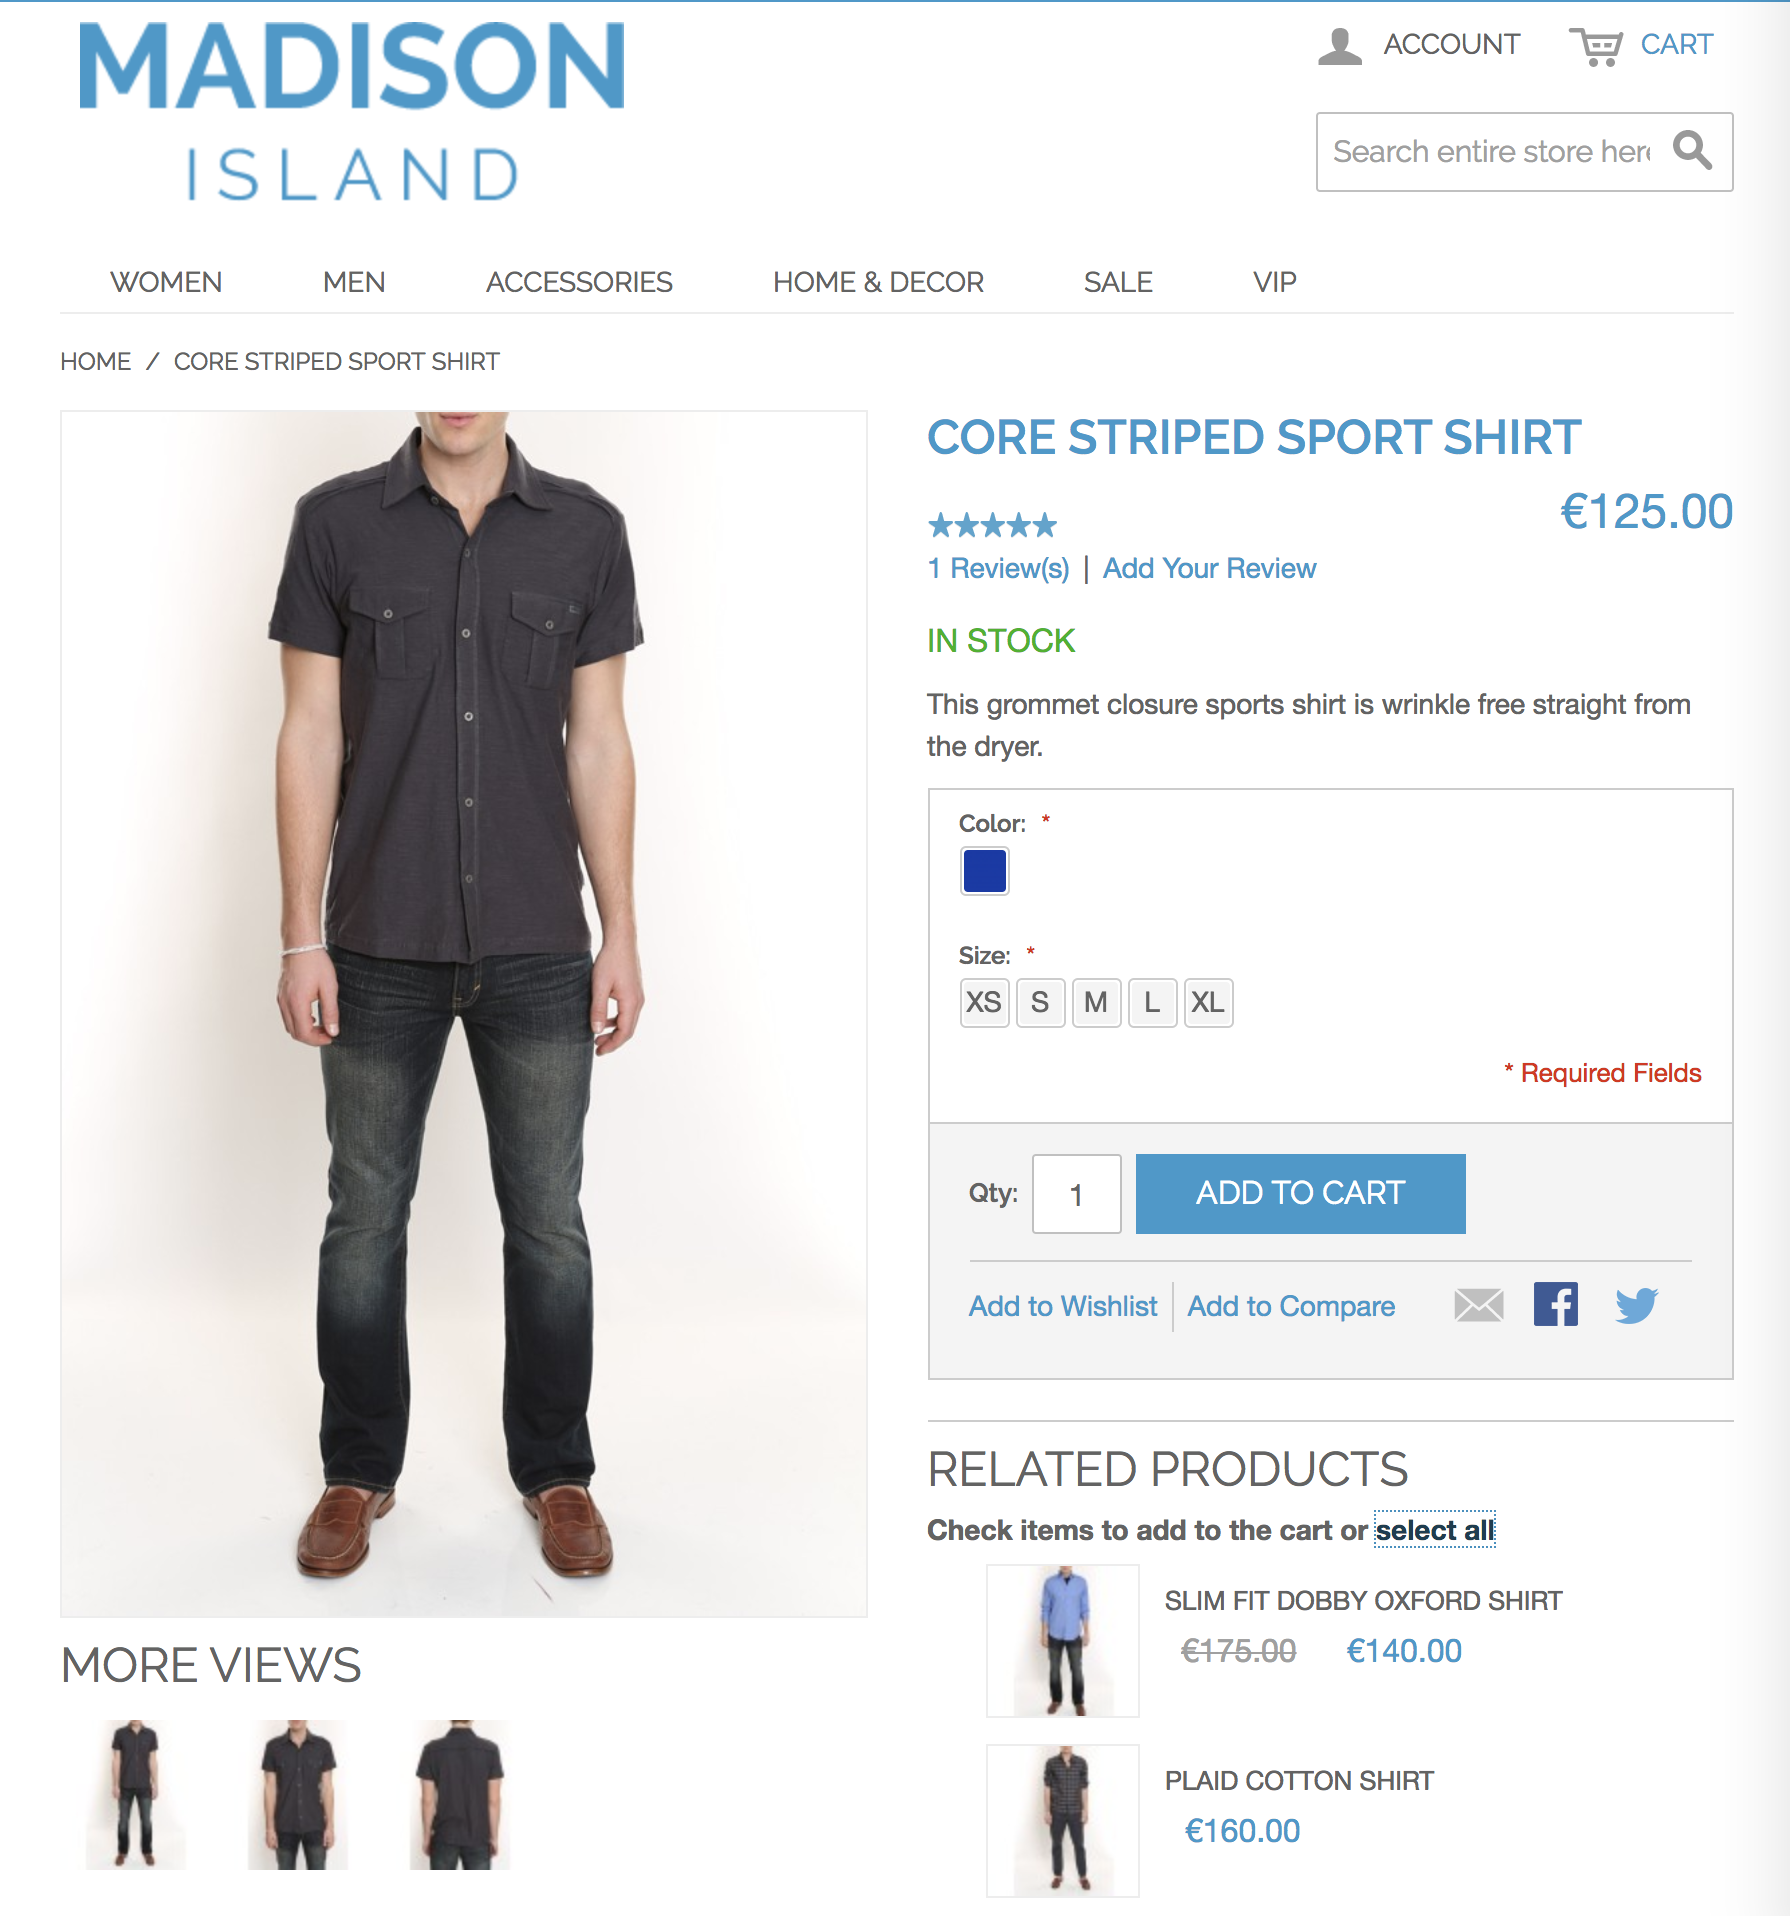
\includegraphics[height=8cm]{images/madison/product-detail2.png}
  \caption{A related product page}
  \label{fig:product-detail2}
\end{figure}
\vspace{0.5cm}

Besides using the simple navigational shortcut available on the related products section, the user can reach a product page in several other ways. The tracking of user interactions could help in establishing a correlation pattern among \textcolor{red}{products}. For instance, users can click on the "back" button in their browser to quickly go to the previous category page and to choose a different item. They can also reach the navigation menu to browser another category, or use the search function on the top bar to perform a global product search. 
Figure \ref{fig:product-search} illustrates the result of the search by the term "blazer" on the search bar within a given product page.

\vspace{0.5cm}
\begin{figure}[H]
  \centering
    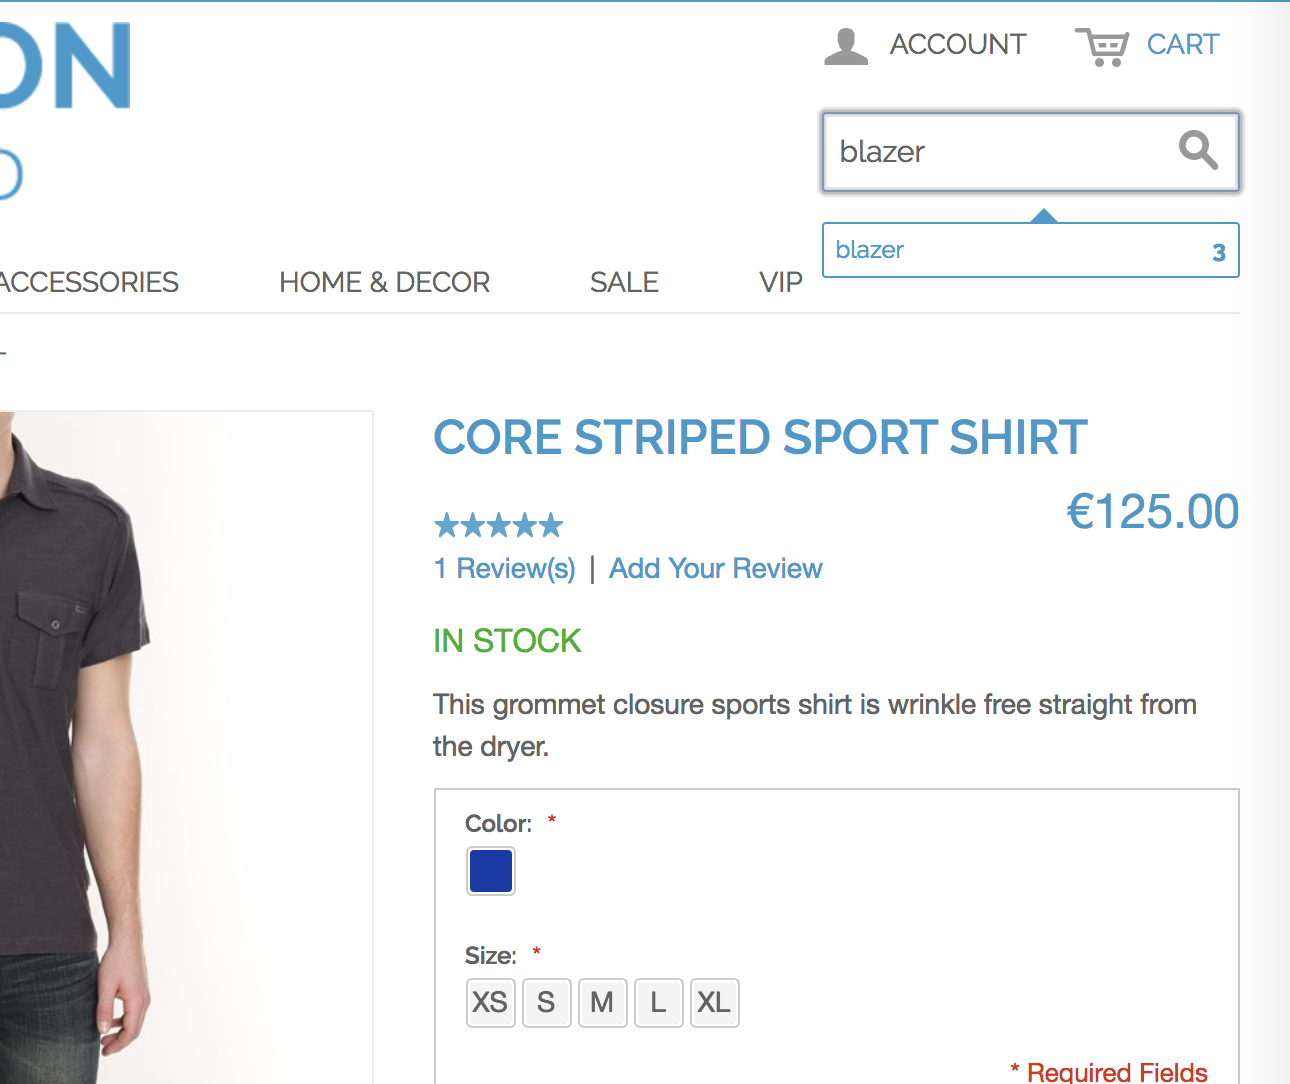
\includegraphics[height=8cm]{images/madison/search.png}
  \caption{Product search bar}
  \label{fig:product-search}
\end{figure}
\vspace{0.5cm}

When the search is performed, the user is taken to the search result page, which lists the products matching searched term. From there, the user can freely browse to any of the available product pages, similarly to the navigation process described for the category listing page. (Figure \ref{fig:search-results})

\vspace{0.5cm}
\begin{figure}[H]
  \centering
    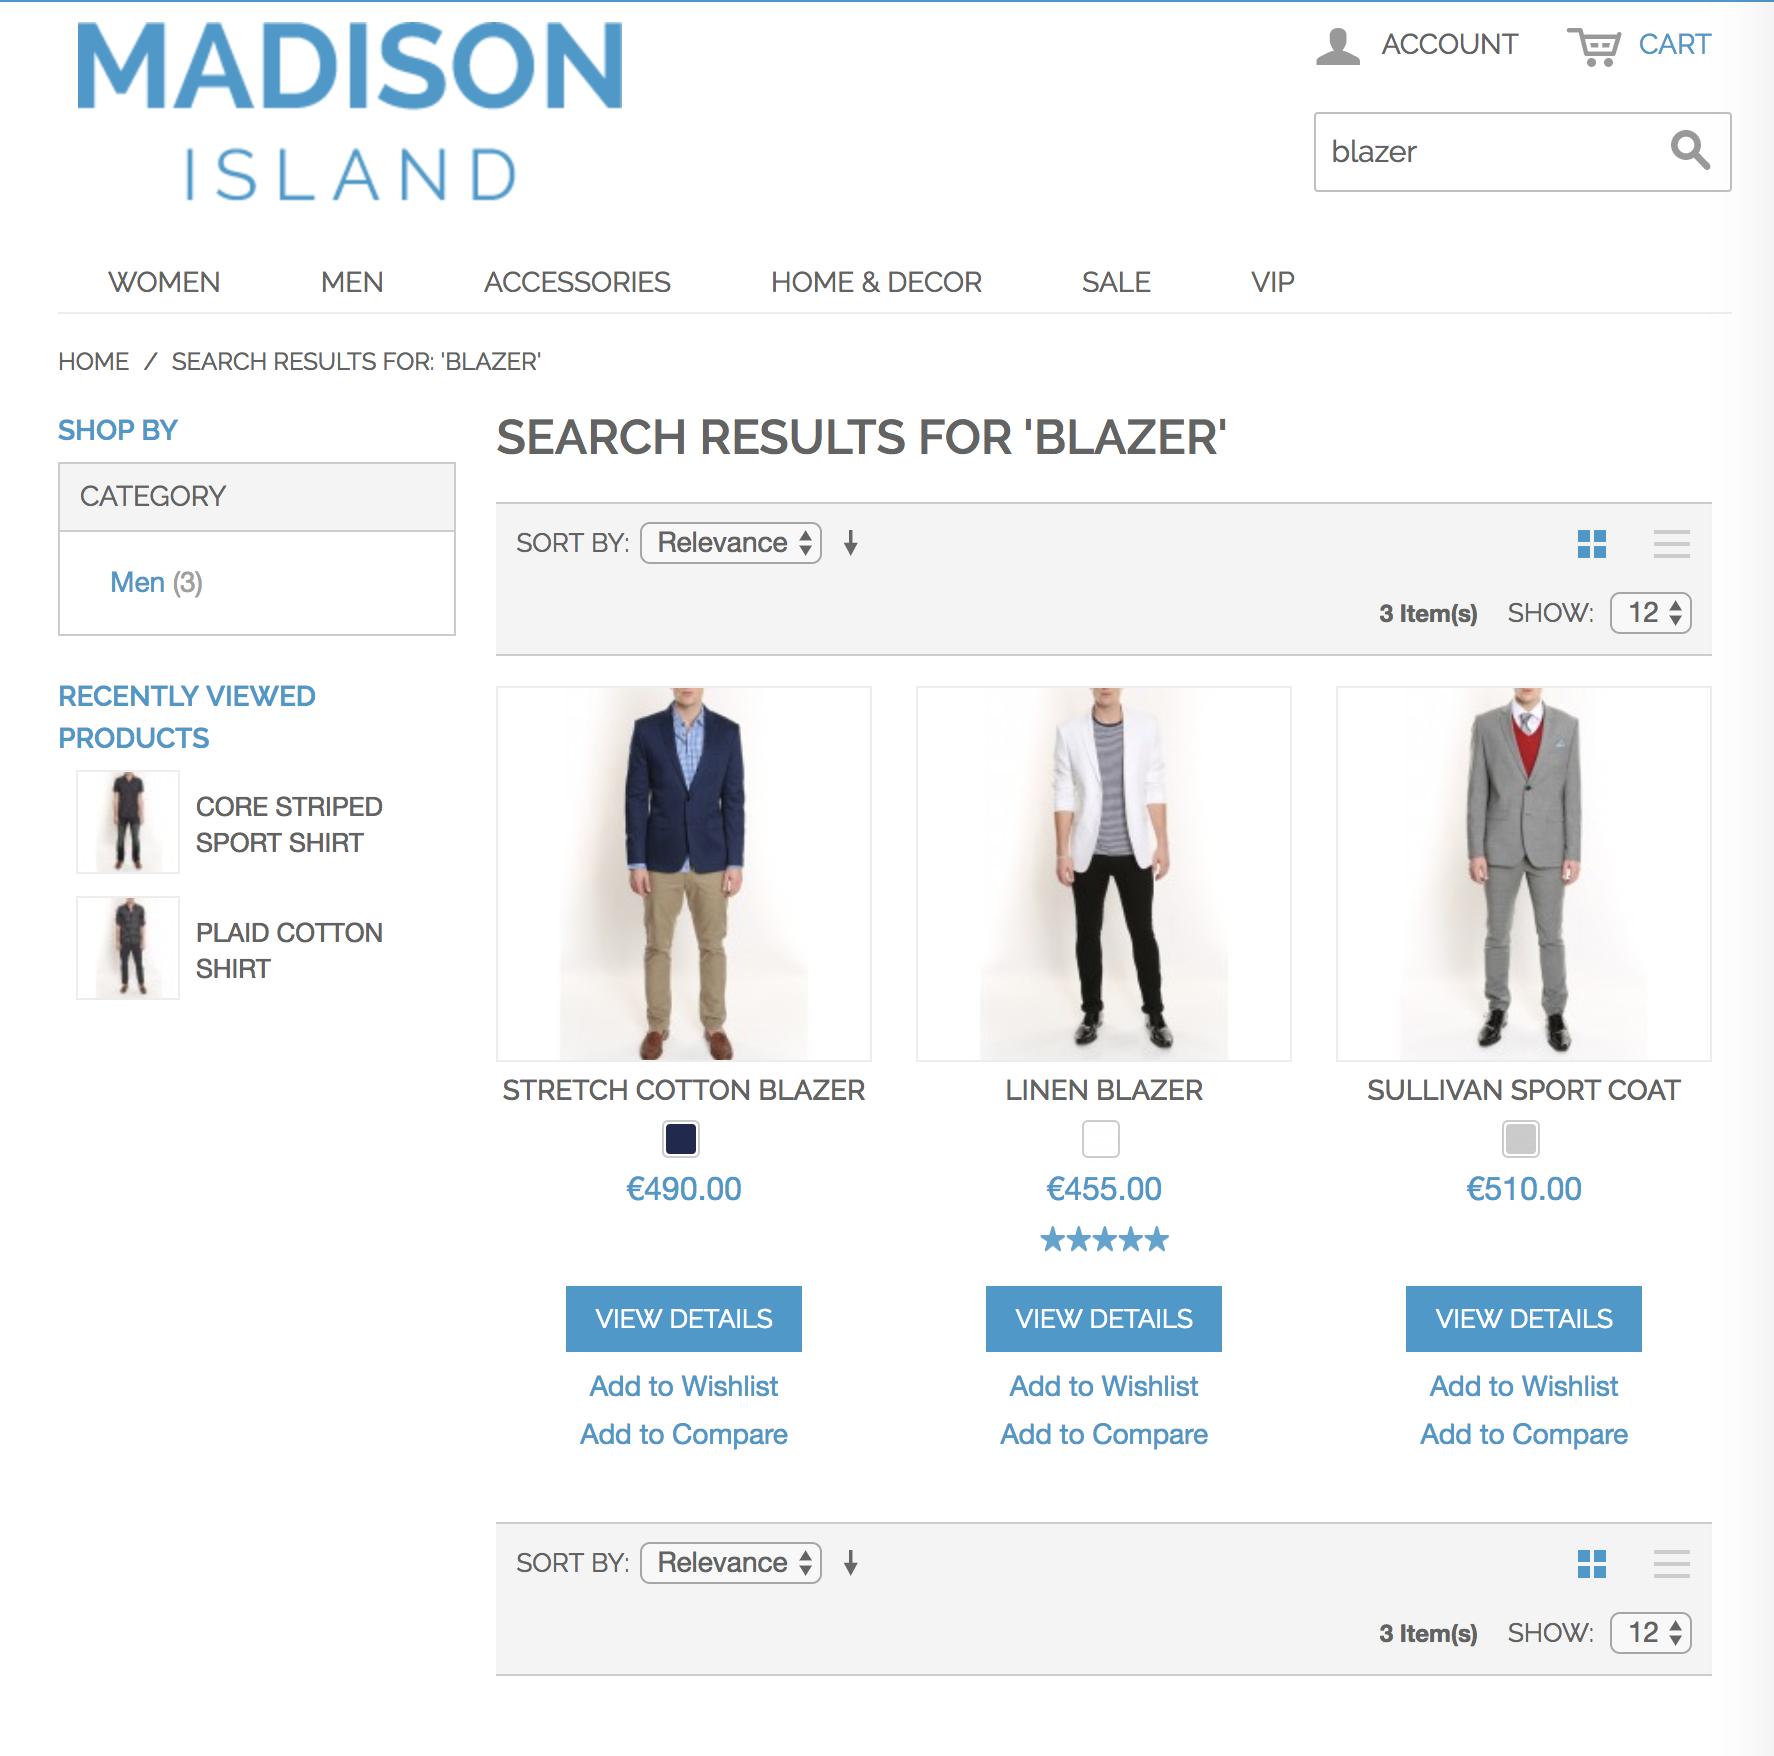
\includegraphics[height=8cm]{images/madison/search-results.png}
  \caption{Search results page}
  \label{fig:search-results}
\end{figure}
\vspace{0.5cm}

At this point, we can update and extend the IFML model shown in Figure \ref{fig:ifml1} according to the new notions and interactions that have been described so far.

\vspace{0.5cm}
\begin{figure}[H]
  \centering
    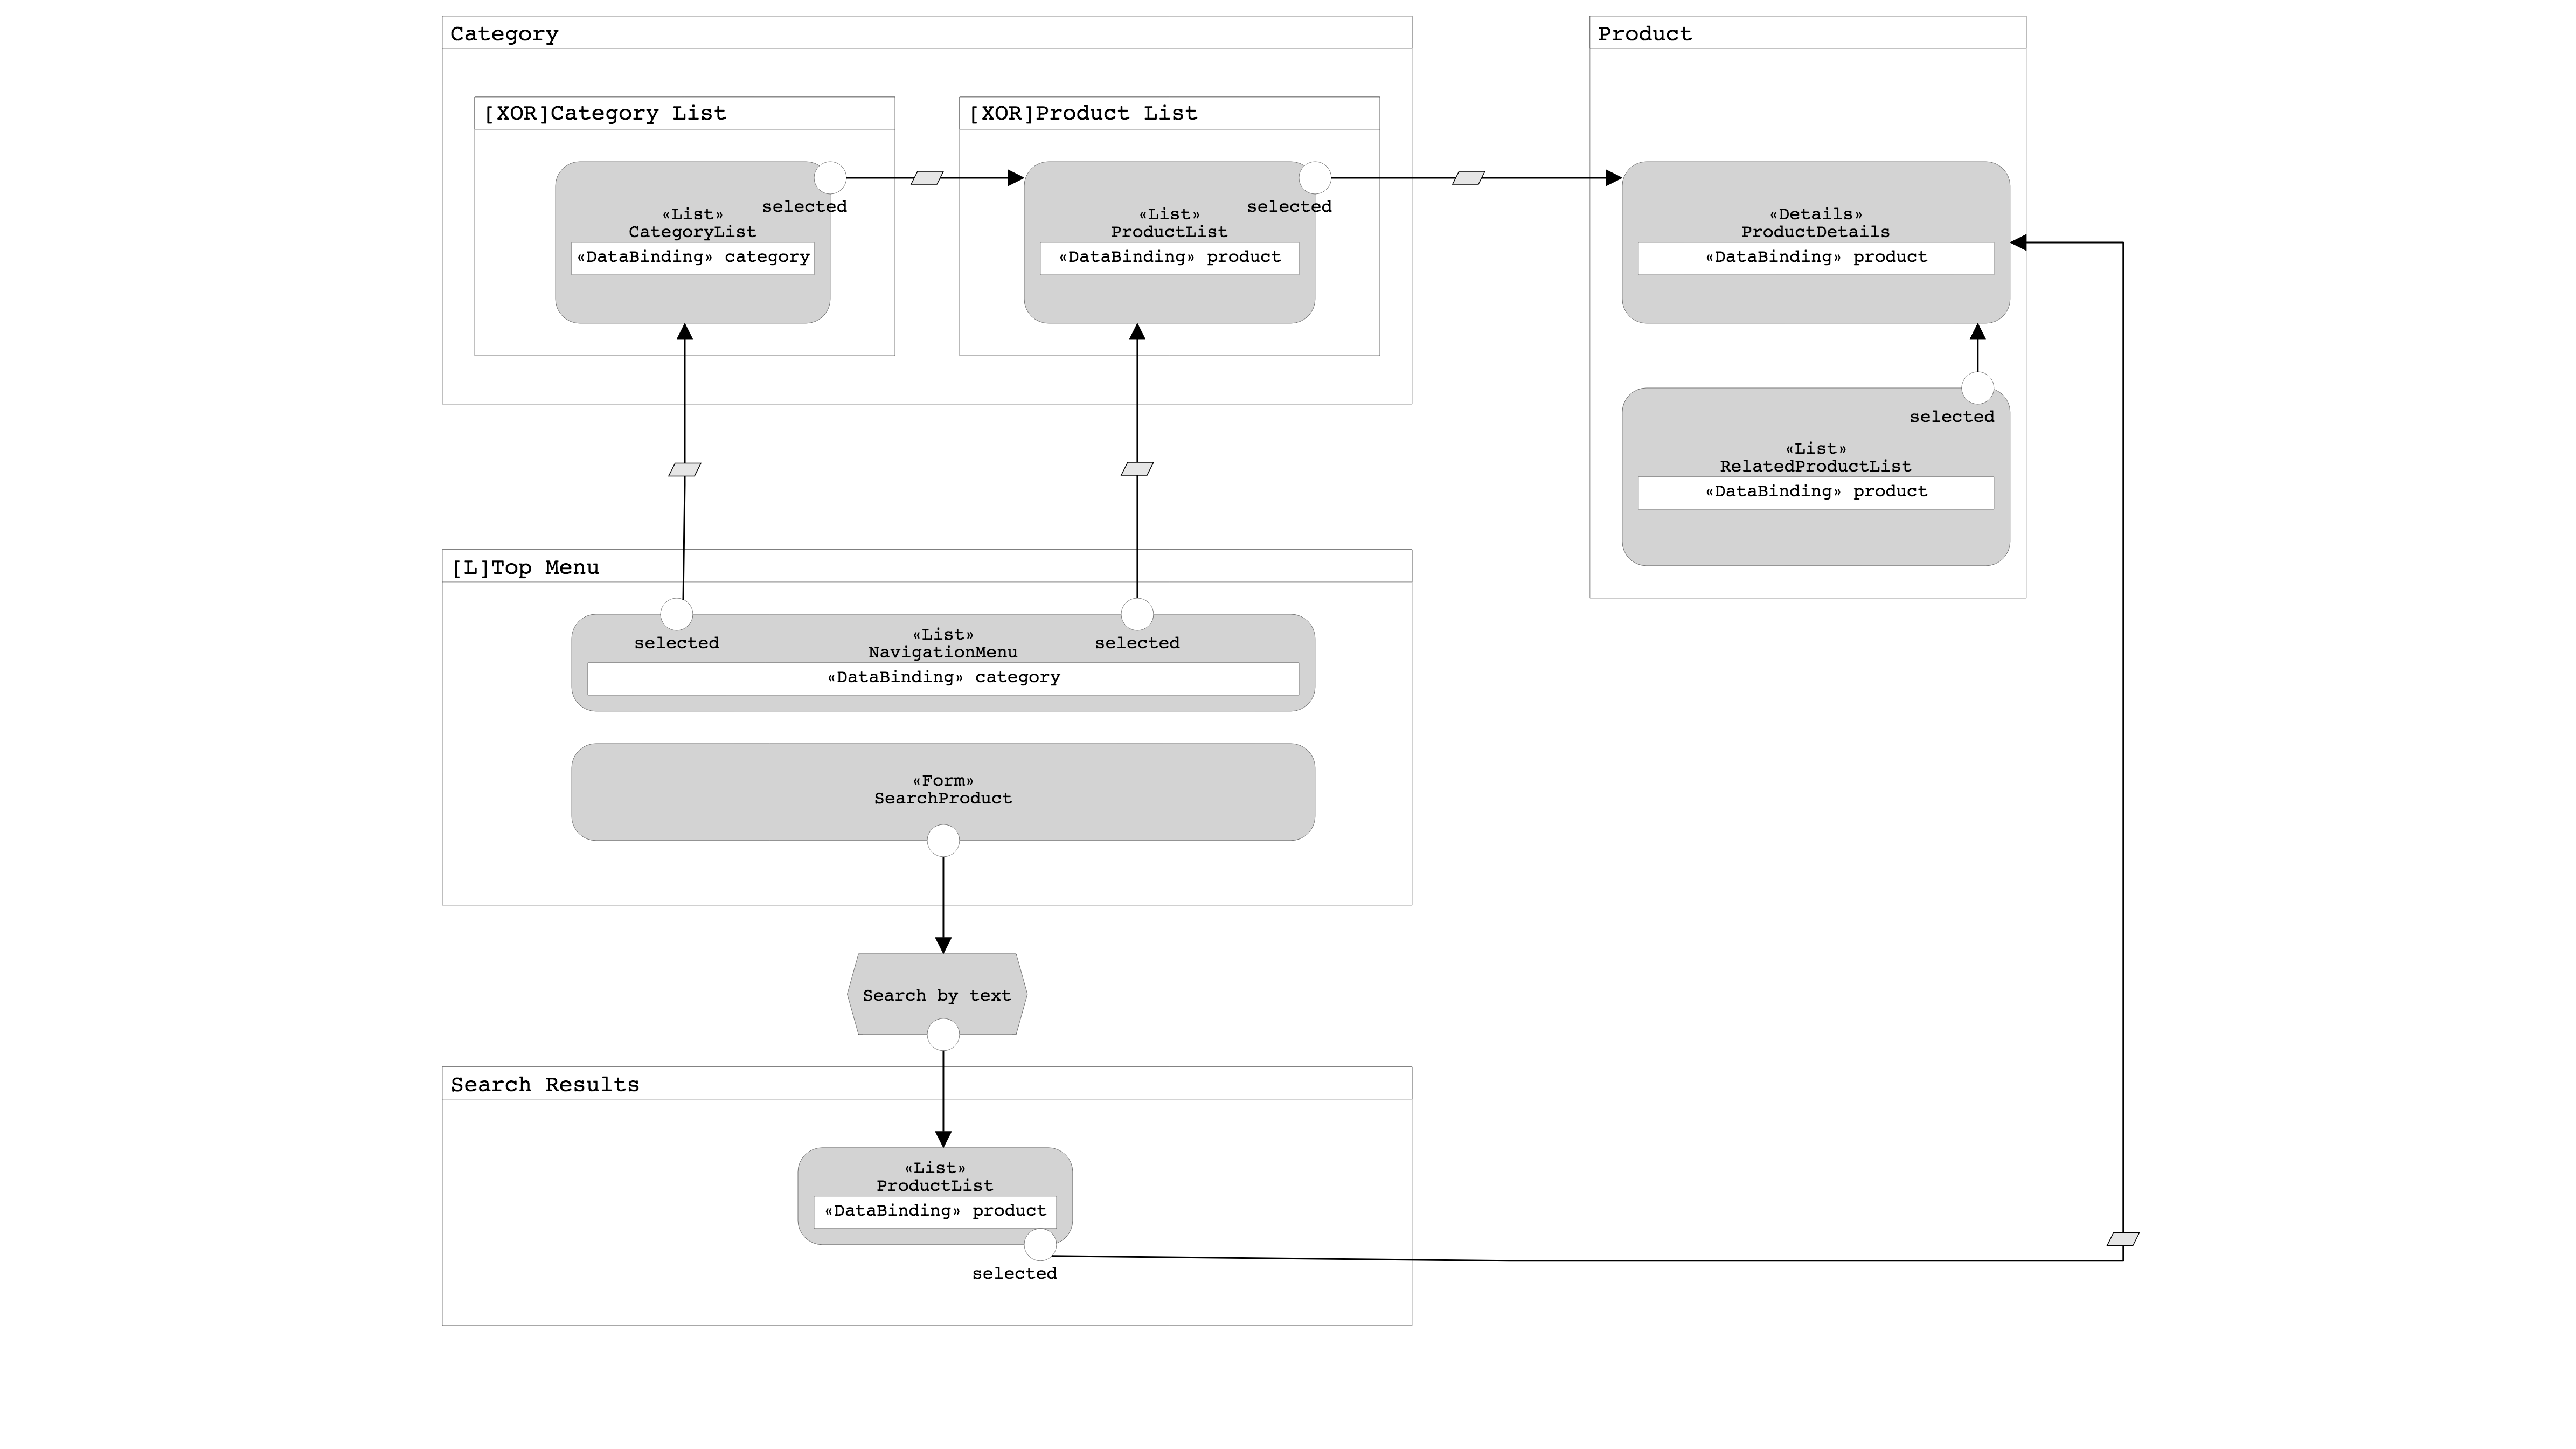
\includegraphics[width=16cm]{images/madison/ifml2.png}
  \caption{Updated IFML representation of the navigational behavious}
  \label{fig:ifml2}
\end{figure}
\vspace{0.5cm}

These new navigational paths are represented in the application server access log in the following manner: 

\vspace{0.5cm}
\begin{center}
  \begin{tabular}{|c|p{3cm}|c|p{6cm}|}
  \hline
  \multicolumn{4}{|c|}{Application Server Access Log}\\ \hline
  \textbf{ID}&\textbf{Page}&\textbf{IFML}&\textbf{Log Entry}   \\ \hline
  1&\textit{"Plaid Cotton Shirt"} Product Page&Product&\em[04/Dec/2017:06:37:06 +0000] 
  "GET /men/shirts/plaid-cotton-shirt-476.html" 200 0 - 29505
  \\ \hline
  2&\textit{"Core Striped Sport Shirt"} Product Page &Product&\em [04/Dec/2017:06:37:15 +0000] "GET /core-striped-sport-shirt-551.html" 200 0 - 29505
  \\ \hline
  3&\textit{"Plaid Cotton Shirt"} Product Page &Product&\em[04/Dec/2017:06:37:21 +0000] "GET /men/shirts/plaid-cotton-shirt-476.html" 200 0 - 29505
  \\ \hline
  5&\textit{"Tees Knits And Polos"} Category Page &Category&\em[04/Dec/2017:06:38:06 +0000] "GET /men/tees-knits-and-polos.html" 200 0 - 29505
  \\ \hline
  6&\textit{"Blazer"} Search By Term&Search Results&\em[04/Dec/2017:06:38:20 +0000] "GET /catalogsearch/result/?q=blazer" 200 0 - 29505
  \\ \hline
  7&\textit{"Stretch Cotton Blazer"} Product Page &Product&\em[04/Dec/2017:06:38:43 +0000] "GET /stretch-cotton-blazer-587.html" 200 0 - 29505
  \\ \hline
  \end{tabular}
  \end{center}
\vspace{0.5cm}

The sequence of actions as seen in this log reveals that the user browsed from one product to another, taking advantage of the related product links (ID 2). In fact, the target URL does not include any category path beside the URL key related to the product, which indicates a direct access. The entries 3 and 4 illustrate the journey of an user who has clicked on the browser back button and has performed the same actions again. The last three recorded actions show, respectively, a direct access to a category page through the navigational menu, a search by the \textit{"blazer"} term as per the previous example, and the related redirection to the product page.

\newpage
\section{IoT behavior profiling}

As mobile devices surpass desktop computers in driving purchases and in enriching behaviour data, location and proximity tracking becomes a valuable tool for brands and stores. In the following subsections, we analyse two possible scenarios of customer interaction in the physical world based on the recording and reporting capabilities of IoT devices. Such data would then be collected together with other web-based information \ref{beacons} to form a comprehensive behavioral data stream that could leverage for generating tailored customizations of the Madison eCommerce portal.

\subsection{Apple iBeacon technology and Estimote Beacons overview}

The IoT device chosen to illustrate the scenarios related to the behavioral modeling would be the Estimote Beacons, which use Apple iBeacon technology and are compatible with iBeacon-enabled Apple products and applications.

The company from Cupertino jumped first on the beacon bandwagon by publishing in 2013 a detailed specification (IDs, transmission intervals, etc.) for developing the iBeacon protocol, which in turn allowed vendors, such as Estimote, to ship iBeacon-compatible hardware transmitters worldwide.

\vspace{0.5cm}
\begin{figure}[H]
  \centering
    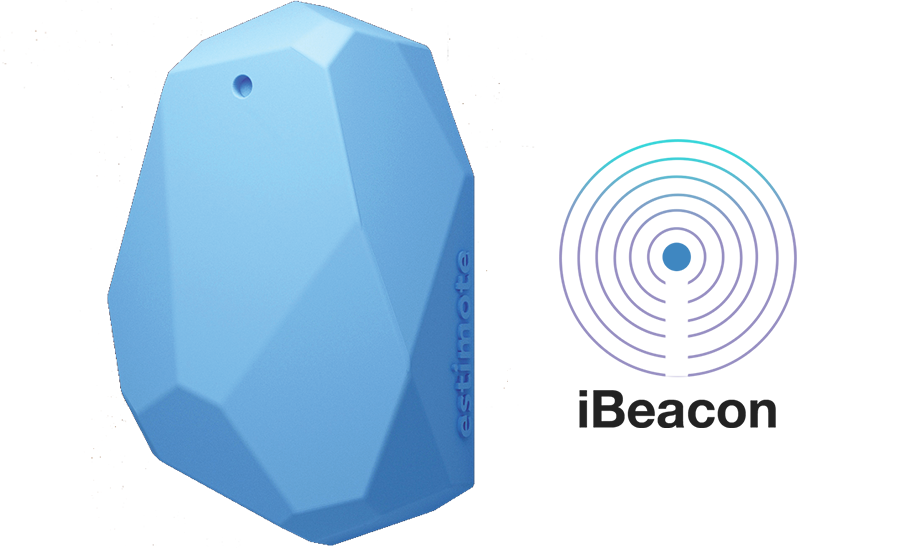
\includegraphics[width=16cm]{images/ibeacon.png}
  \caption{An Estimote iBeacon compatible device}
  \label{fig:estimote-beacon}
\end{figure}
\vspace{0.5cm}

As described in Section \ref{beacons}, a beacon can simply be seen as a lighthouse that broadcasts information in certain intervals and at a defined power, leveraging Low Energy Bluetooth connection. In the case of iBeacons, the information sent to listening mobile devices would contain:


\begin{itemize}
  \item The Universal Unique ID (UUID), which is globally unique. Example: de2b45ae-ed98-11e4-3432-78616d6f6f6d
  \item The Major ID, which uniquely identifies our customer’s system: e.g. 51314
  \item The Minor ID, which reports the exact location or object (in our case, the spot): e.g. 23369
\end{itemize}

Unlike QR and NFC communication, the customer needs to have an app installed on his phone to receive this one-way data stream. Technically, the app obeys only to "its" iBeacons, i.e., those with fitting UUID, Major and Minor IDs \textcolor{red}{looking for a match}. When that happens, the app can react accordingly. Such mechanism ensures that only the installed app can track users as they passively walk around the transmitters. 

In other words, the phone OS will keep listening for beacons even if the app is not running, and even if the phone is locked or rebooted. Once either an “enter” or and “exit” event happens, the OS will launch the app into the background (if needed) and let it execute, for a few seconds, some code to handle the event.

\subsection{Proximity Marketing}
\label{ssection:proximity-marketing}

Proximity Marketing is an efficient tool not only for discovering and engaging potential customers, but also fro better targgeting existing ones. This marketing technique operates in a given physical location by leveraging the IoT ecosystem to promote products and services.  This communication channel acts on a clear target: all the customers close to or within an area covered by the diffusion devices.

Such innovative form of relationship marketing aims to activate and involve users by drawing their attention at the right time and in the right place, creating more intense and stimulating shopping experiences.

In this work, we will focus on a basic scenario where the recognition of proximity in the physical world does not directly trigger an immediate action to grab customer attention, but instead is limited to the silent tracking of the event as well as the automatic recording of data on a specific web server.

We start by defining a possible allocation of items for a "Madison Island" retail store which, resembles the catalog presented on its website.

\vspace{0.5cm}
\begin{figure}[H]
  \centering
    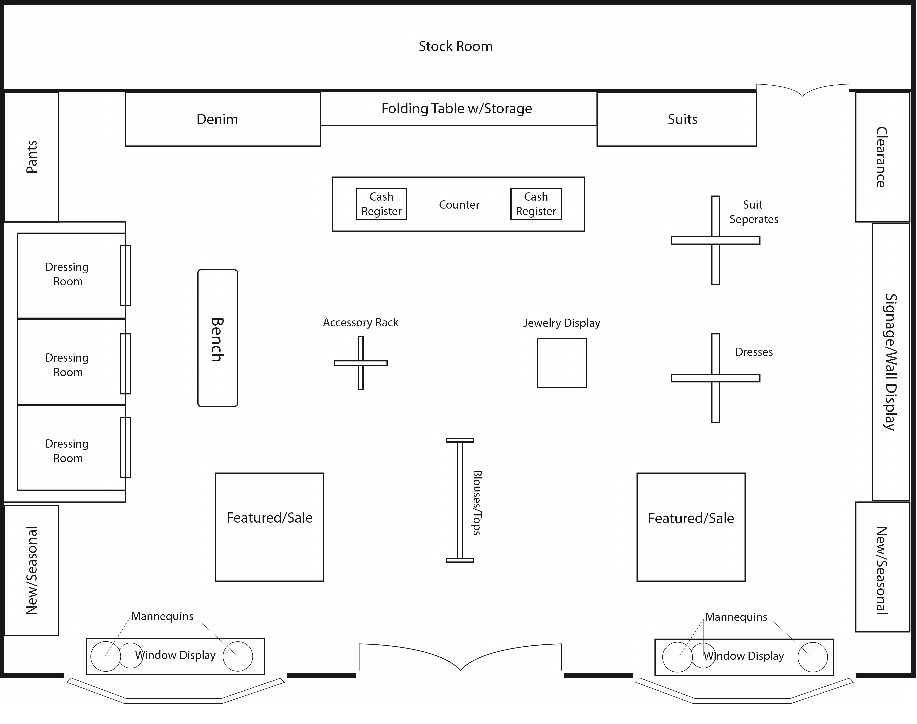
\includegraphics[width=16cm]{images/madison/retail-map.jpg}
  \caption{Madison Island brick-and-mortar store map}
  \label{fig:retail-map}
\end{figure}
\vspace{0.5cm}

Each label described in Figure~\ref{fig:retail-map} represents a specific category of the website whereas the color of the label indicates the parent category to which the products belong. More specifically:

\begin{itemize}
  \item Red represents the \textbf{Women} category, which maps the content available at \textbf{/women.html}. 
  \item Blue represents the \textbf{Men} category, which maps the content available at \textbf{/men.html}.
  \item Purple represents the \textbf{Home \& Decor} category, which maps the content available at \textbf{/home-decor.html}. 
  \item Orange represents the \textbf{Accessories} category, which maps the content available at \textbf{/accessories.html}. 
\end{itemize}

As a customer walks around the physical shop, the Madison Island mobile app looks for a predefined set of beacon regions. Whenever the device either enters or exits each region, the app registers proximity data and tracks the aisles (regions) visited or not by the customer.

In this scenario, the following image illustrates what would be a suitable Estimote beacon allocation for the store:

\vspace{0.5cm}
\begin{figure}[H]
  \centering
    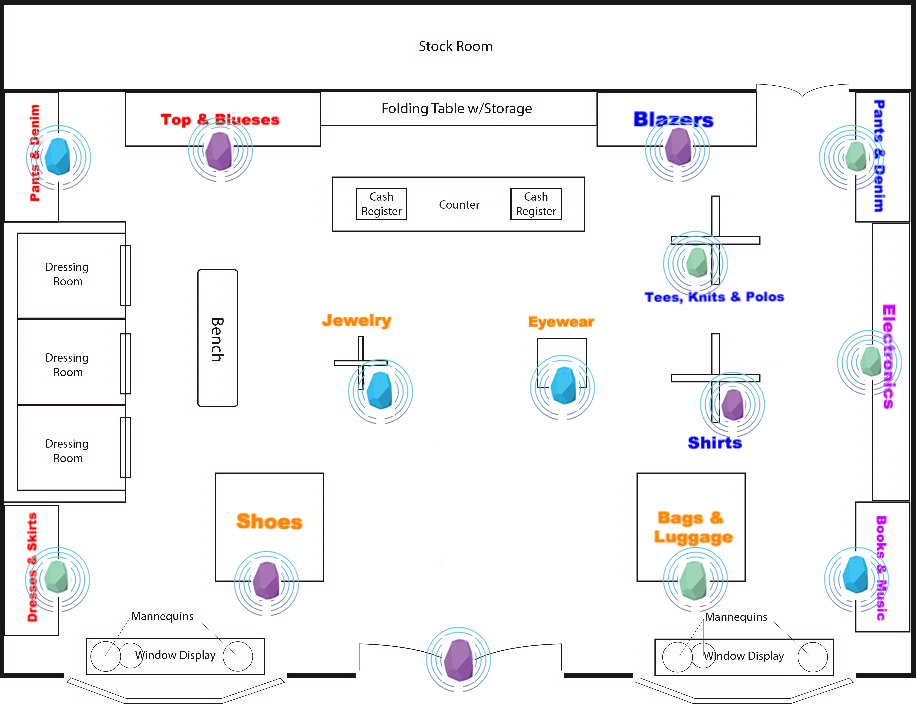
\includegraphics[width=16cm]{images/madison/retail-map-beacon.jpg}
  \caption{Madison Island brick-and-mortar store with Estimote beacons allocation}
  \label{fig:beacons-map}
\end{figure}
\vspace{0.5cm}

Depending on the business use case, the mobile app can either send an event to the listening server whenever the user crosses a region boundary, or submit a single event with a full list of regions and their minimum proximities detected during the visit. 

Due to the behavioral profiling nature of this activity, we assume that the app does the latter, detecting all the entering and leaving of each virtual fence and activating a \textit{ranging} procedure that detects proximity information based on the strenght of the Bluetooth signal. \cite{region-monitoring-apple}.

Once the shoppers leaves the physical store, the app performs a single data push to a REST API endpoint with all the tracked data.

From a technical perspective, all these operations are accomplished leveraging the Estimote iOS-SDK \cite{estimote-ios-sdk}, which allows the developer to quickly define regions and ranges for each beacon and facilitates the tracking of the actual proximity to beacon through the ranging process.

As an example, the JSON payload sent from the app to the REST endpoint for an hypothetical customer 3045678 (e.g. \textbf{POST /users/3045678/sessions}) would have the following structure:


\vspace{0.5cm}
\begin{lstlisting}[language=json,firstnumber=1]
  {
    "data":{
       "customerId":3045678,
       "storeId":8784,
       "storeLabel" : "Madison1",
       "sessionId" : "89376f84-065b-11e8-ba89-0ed5f89f718b"

       "sessionRegions":[
             {
                "regionId: : 156,
                "regionLabel":"store-entrance",
                "detectionCount":2,
                "maxSecondsInRegion": 5,
                "maxProximity":"unknown",
                "firstDetectionTimestamp":"2018-02-21T18:09:07Z",
                "lastDetectionTimestamp":"2018-02-21T18:16:02Z",
                "beaconData" : {
                  "uuid":"0686a88e-fed6-11e7-8be5-0ed5f89f718b",
                  "majorId":2553,
                  "minorId":79
                }
             },
             {
                "regionId: : 645,
                "regionLabel":"shoes",
                "detectionCount":1,
                "maxSecondsInRegion": 24,
                "maxProximity":"near",
                "firstDetectionTimestamp":"2018-02-21T18:09:20Z",
                "lastDetectionTimestamp":"2018-02-21T18:09:20Z",
                "beaconData" : {
                  "uuid":"0686a88e-fed6-11e7-8be5-0ed5f89f718b",
                  "majorId":19029,
                  "minorId":49
                }
             },
             {
                "regionId" : 6875,
                "regionLabel":"jewelry",
                "detectionCount":1,
                "maxSecondsInRegion": 15,
                "maxProximity":"far",
                "firstDetectionTimestamp":"2018-02-21T18:10:15Z",
                "lastDetectionTimestamp":"2018-02-21T18:10:15Z",
                "beaconData" : {
                  "uuid":"0686a88e-fed6-11e7-8be5-0ed5f89f718b",
                  "majorId":38415,
                  "minorId":59
                }
             },
             {
                "regionId" : 2563,
                "regionLabel":"blazers",
                "detectionCount":1,
                "maxSecondsInRegion": 195,
                "maxProximity":"immediate",
                "firstDetectionTimestamp":"2018-02-21T18:11:01Z",
                "lastDetectionTimestamp":"2018-02-21T18:11:01Z",
                "beaconData" : {
                  "uuid":"0686a88e-fed6-11e7-8be5-0ed5f89f718b",
                  "majorId":25911,
                  "minorId":27
                }
             },
             {
                "regionId" : 456,
                "regionLabel":"tees-knits-polos",
                "detectionCount":1,
                "maxSecondsInRegion": 10,
                "maxProximity":"far",
                "firstDetectionTimestamp":"2018-02-21T18:14:56Z",
                "lastDetectionTimestamp":"2018-02-21T18:14:56Z",
                "beaconData" : {
                  "uuid":"0686a88e-fed6-11e7-8be5-0ed5f89f718b",
                  "majorId":42037,
                  "minorId":36
                }
             },
             {
                "regionId" : 998,
                "regionLabel":"bags-and-luggage",
                "detectionCount":1,
                "maxSecondsInRegion": 7,
                "maxProximity":"far",
                "firstDetectionTimestamp":"2018-02-21T18:15:12Z",
                "lastDetectionTimestamp":"2018-02-21T18:15:12Z",
                "beaconData" : {
                  "uuid":"0686a88e-fed6-11e7-8be5-0ed5f89f718b",
                  "majorId":37931,
                  "minorId": 85
                }
             }
          ]
    }
 }
  \end{lstlisting}
\vspace{0.5cm}


The above example session shows an evident preference for "Blazer" items, and a slight interest in "Shoes" items. More precisely, the "Blazer" region registered a session that lasted over 3 minutes and that was the closest to a beacon.  

\subsection{Customer Rewards}

Besides allowing proximity based marketing, beacon technology can also be used to reward customers for particular actions based on geolocalization data. Such rewards could increase brand engagement, enhancing customer loyalty and fostering lasting customer relationships. 

Achieving such results is possible by extending the set of actions that enable customers to earn bonuses and discounts on the website (newsletter subscriptions, minimum order amount, etc..) to activities performed in the physical world, including the simple act of visiting and walking around the brick-and-mortar store.

For example, the brand can rank customers by the amount of time spent at each Madison Retail shop, rewarding them with monthly offers tailored according to their purchases. The brand can also focus on offering special offers on the website to the customers that visited a retail store in a specific time span such as Christmas.

For our Madison Island example, we are considering a scenario where customers are rewarded with a fixed amount of points on their online account if they scan three QR codes from in-store products. Specifically, when the beacon detects their entrance into the store, the mobile app pushes a CheckPoints notification to the customer, inviting them to scan codes of items available in the shop. Once the scans are correctly performed within a session, the mobile app pushes the information to the same REST API presented in the previous chapter, which then stores the data.

\vspace{0.5cm}
\begin{figure}[H]
  \centering
    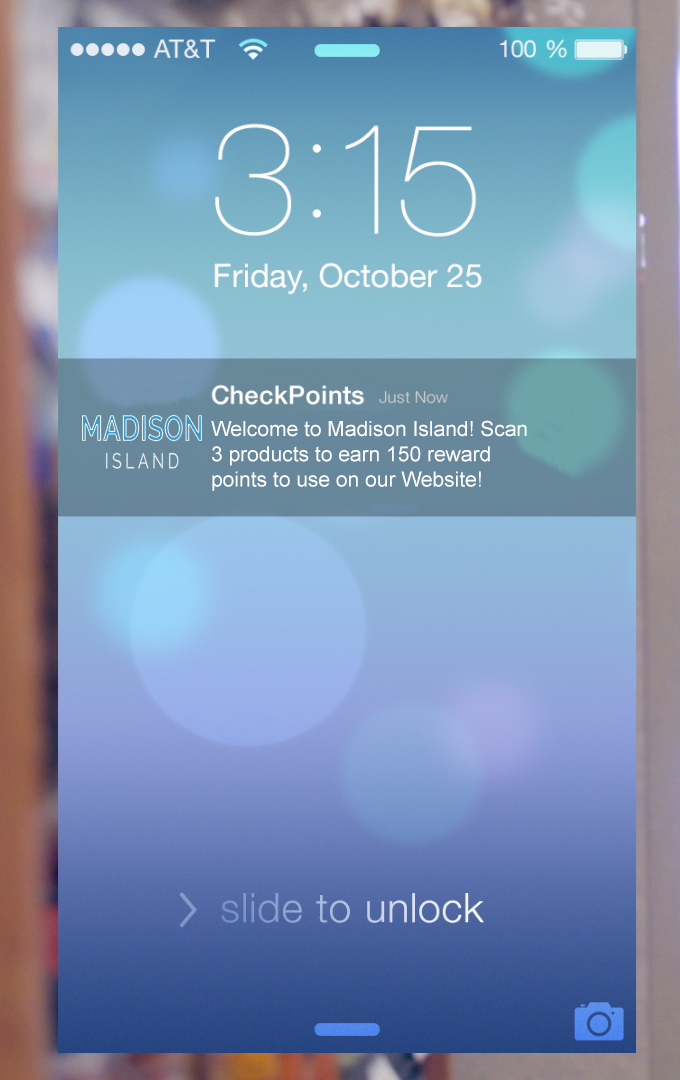
\includegraphics[width=8cm]{images/madison-push-reward-points.jpg}
  \caption{Madison Island mobile app push notification example}
  \label{fig:mobile-app-push-notification}
\end{figure}
\vspace{0.5cm}


The JSON payload sent to the server (e.g. \textbf{POST /users/3045678/scans}) after each succesful scan would then have a structure similar to the following one:
 
\vspace{0.5cm}
\begin{lstlisting}[language=json,firstnumber=1]
  {
    "data":{
       "customerId":3045678,
       "storeId":8784,
       "storeLabel" : "Madison1",
       "sessionId" : "89376f84-065b-11e8-ba89-0ed5f89f718b"
       "sessionDuration" : 456,
       "sessionActions": [{
          "userAgent" : "Iphone 6s",
          "scannedItems":
            [{
              "barcode":"042100005264",
              "name" : "Elizabeth Knit Top-Red-S"
              "sku": "wbk012c-Red-S"    
            },
            {
              "barcode":"042100005931",
              "name" : "Plaid Cotton Shirt-Khaki-L"
              "sku": "msj006c-Khaki-L"    
            },
            {
              "barcode":"042100007717",
              "name" : "Broad St Saddle Shoes"
              "sku": "shm00110"    
            }
            ]
      }]
    }
 }
  \end{lstlisting}
\vspace{0.5cm}


\vspace{0.5cm}
\begin{figure}[H]
  \centering
    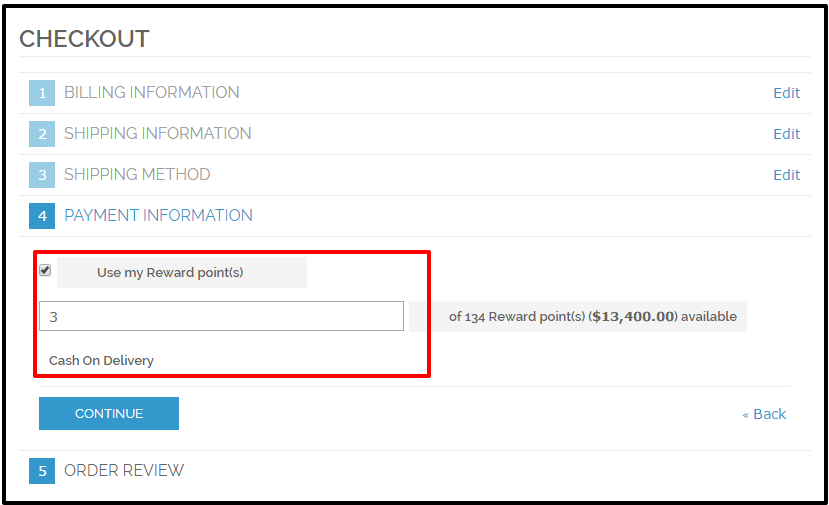
\includegraphics[width=12cm]{images/loyalty-reward-points.png}
  \caption{Madison Island loyalty program usage during checkout}
  \label{fig:loyalty-points}
\end{figure}
\vspace{0.5cm}

Similarly to the process outlined in \ref{ssection:proximity-marketing}, the product data collected when customers scan codes during their visits to the physical store will potentially be converted into reward points to be used by the same customer on the website.  

